
\chapter{Resultados}
Nessa seção apresentamos os principais resultados na elaboração deste trabalho. Eles são referentes as análises das bases de dados, das funções de custos, codificação de entropia e alocação dinâmica de bits no desempenho do modelo. 

%A nossa hipótese é que o desempenho do autoencoder está relacionado com características da entropia da base de dados utilizado no treinamento.

\section{Análise da Base de Dados}

Treinamos 5 modelos do autocodificador para cada base de dados apresentada em \ref{list:bds} e usando a função \acrshort{mae} sobre os resíduos como função de custo. Além disso, os seguintes hiperparâmetros da rede foram adotados neste experimento: 

\begin{enumerate}
	\label{enum:hiper_param}
	\item Tamanho do lote: 32; 
	\item Número de lotes de treinamento por época: 38 mil (aproximadamente);   
	\item Número de iterações: 16;
	\item Número de épocas: 1;
	\item Taxa de aprendizado: $5 \times {10}^{-4}$.
\end{enumerate}

Calculamos os valores médios de \acrshort{psnr}, \acrshort{ssim} e \acrshort{msssim} das imagens da Kodak reconstruídas na taxa nominal de 2 bits por pixel. Os resultados estão disponíveis na tabela \ref{table:comp_datasets}.


\begin{table}[htbp]
	\centering
	\caption[Comparação das bases de dados]{Comparação das bases de dados.}
	\begin{tabular}{|c|c|c|c|}
		\hline
		\textbf{Base de dados} & \textbf{PSNR(dB)}    & \textbf{SSIM}   & \textbf{MS-SSIM}\\\hline
		0            & 25,4268          & 0,6978          & 0,9177           \\\hline
		1            & 31,9458          & 0,9201          & 0,9874           \\\hline
		2            & 34,3622          & 0,9444          & 0,9900           \\\hline
		3            & 32,9632	       & 0,9327          & 0,9890           \\\hline
		\textbf{4}            & \textbf{34,3903} & \textbf{0,9473} & \textbf{0,9913}     
		\\ \hline
	\end{tabular}
	\label{table:comp_datasets}
\end{table}

Conforme esperado, uma base de dados de alta entropia é indicada para treinar o modelo. A hipótese é que essa característica otimiza a rede a aprender padrões não triviais das imagens e evitar o sobre-ajuste do modelo. A base de dados 4, nessa tabela, obteve o melhor resultado, por uma pequena margem em relação à BD2.

As figuras \ref{fig:psnr_db2_db4} \ref{fig:ssim_db2_db4} e \ref{fig:msssim_db2_db4} ilustram os resultados do autocodificador treinado pelas bases de dados 2 e 4 em relação às métricas \acrshort{psnr}, \acrshort{ssim} e \acrshort{msssim} para taxas nominais no intervalo de 0,125 a 2,0 bpp com incrementos constantes de 0,125 bpp. Elas indicam que o modelo treinado pela BD4 apresenta um melhor desempenho. 

\begin{figure}[H]
	\centering
	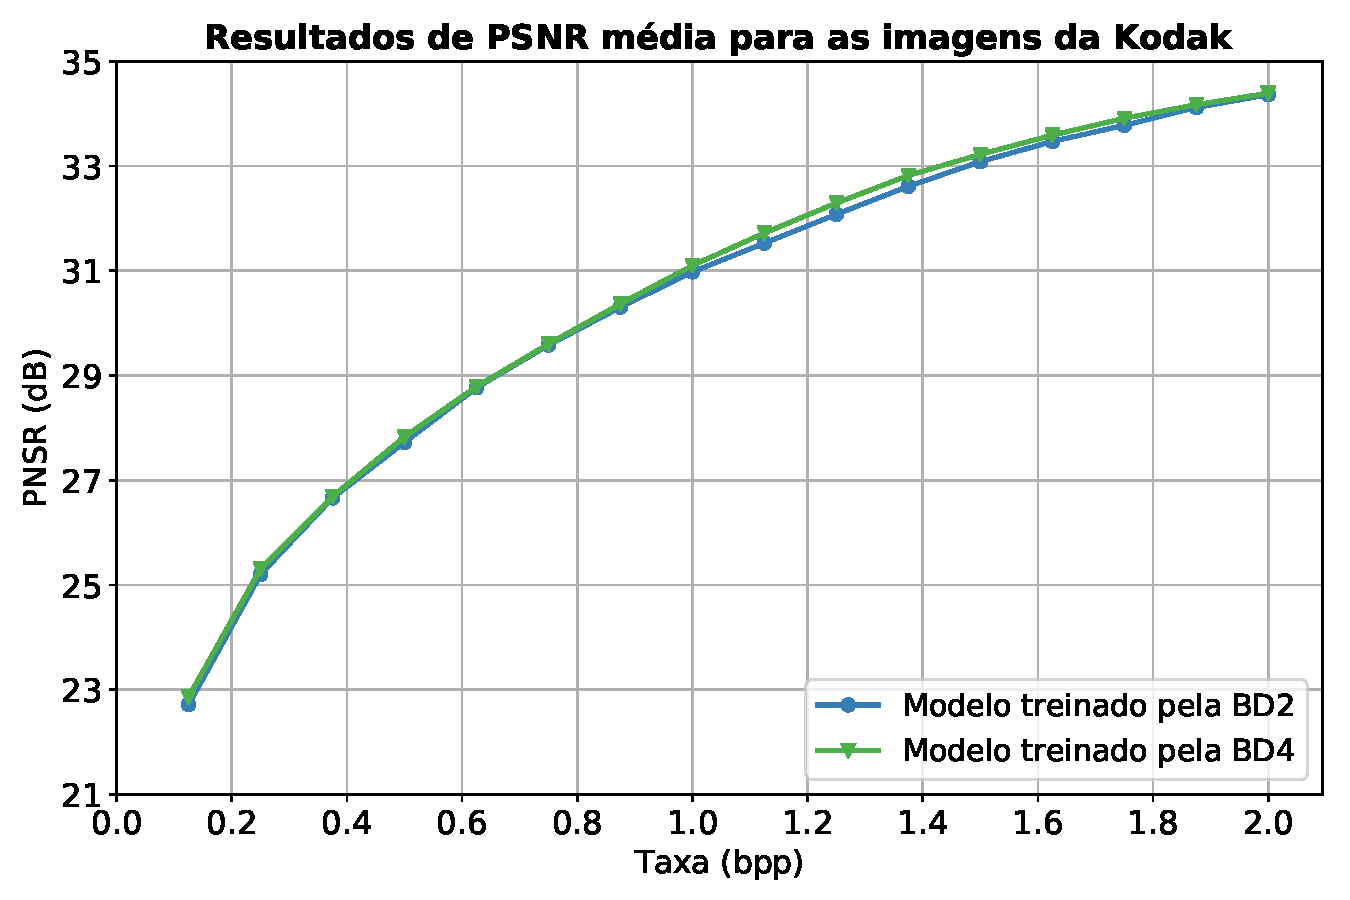
\includegraphics[width=0.9\textwidth]{figuras/psnr_db2_db4.pdf}
	\caption[Comparação dos resultados das bases de dados 2 e 4 em relação à \acrshort{psnr}]{Comparação dos modelos obtidos pelas bases de dados 2 e 4 em relação à \acrshort{psnr} para várias taxas.} 
	\label{fig:psnr_db2_db4}
\end{figure}

\begin{figure}[H]
	\centering
	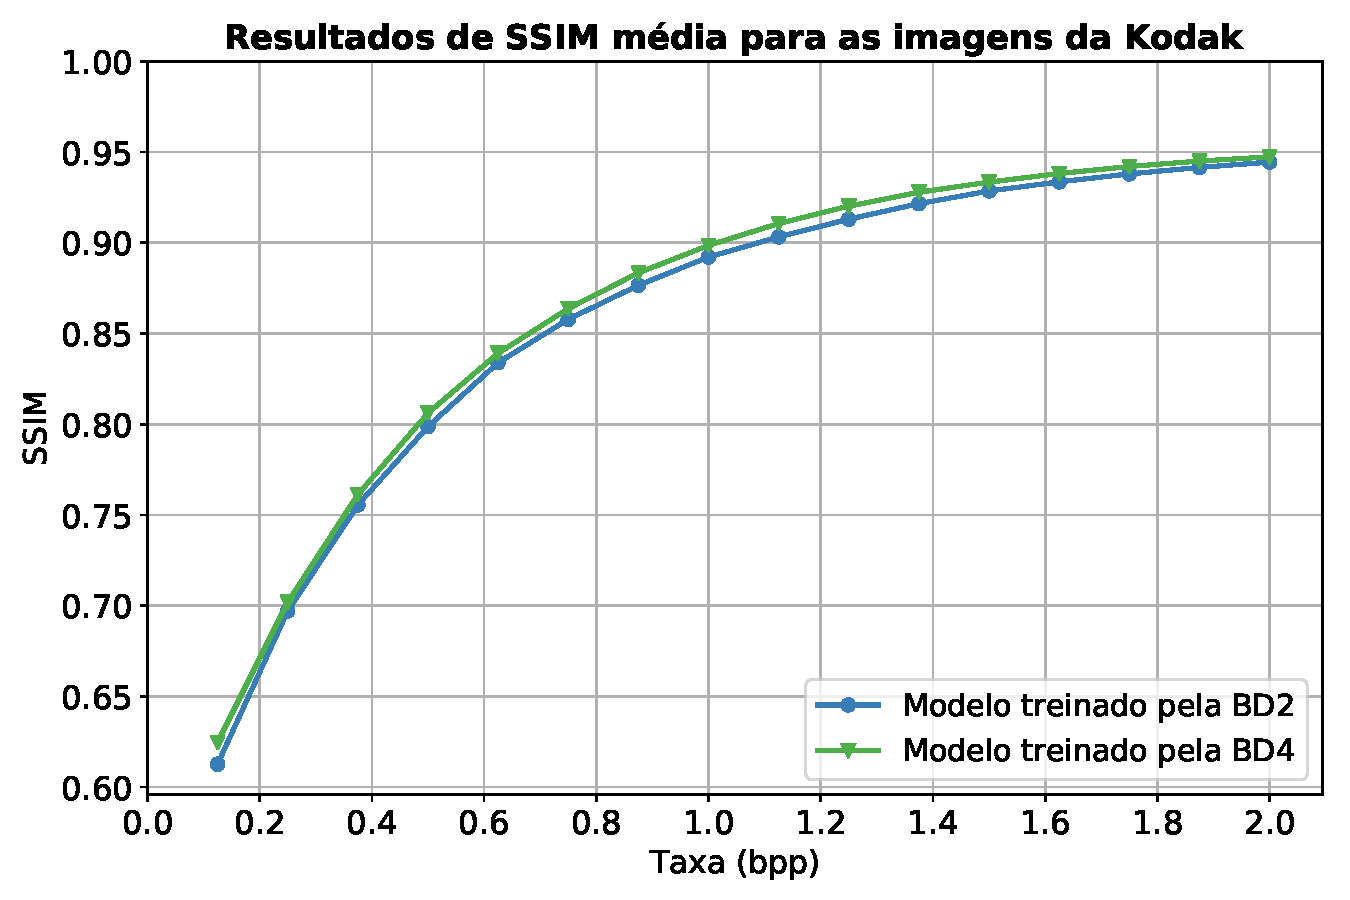
\includegraphics[width=0.9\textwidth]{figuras/ssim_db2_db4.pdf}
	\caption[Comparação dos resultados das bases de dados 2 e 4 em relação à \acrshort{ssim}]{Comparação dos modelos obtidos pelas bases de dados 2 e 4 em relação à \acrshort{ssim} para várias taxas.} 
	\label{fig:ssim_db2_db4}
\end{figure}

\begin{figure}[H]
	\centering
	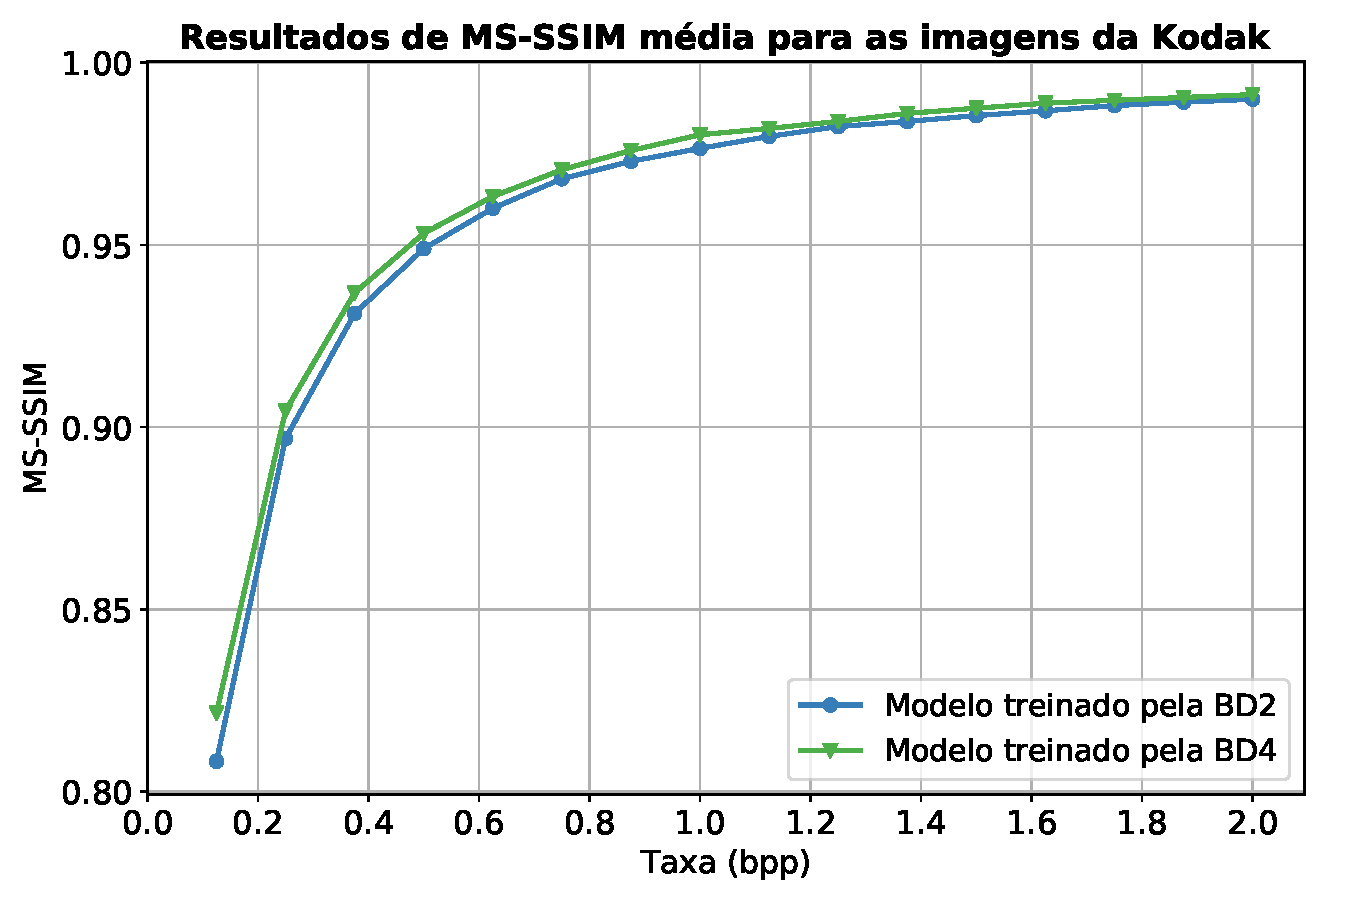
\includegraphics[width=0.9\textwidth]{figuras/msssim_db2_db4.pdf}
	\caption[Comparação dos resultados das bases de dados 2 e 4 em relação à \acrshort{msssim}]{Comparação dos modelos obtidos pelas bases de dados 2 e 4 em relação à \acrshort{msssim} para várias taxas.} 
	\label{fig:msssim_db2_db4}
\end{figure}



%\begin{figure}
%	\centering
%	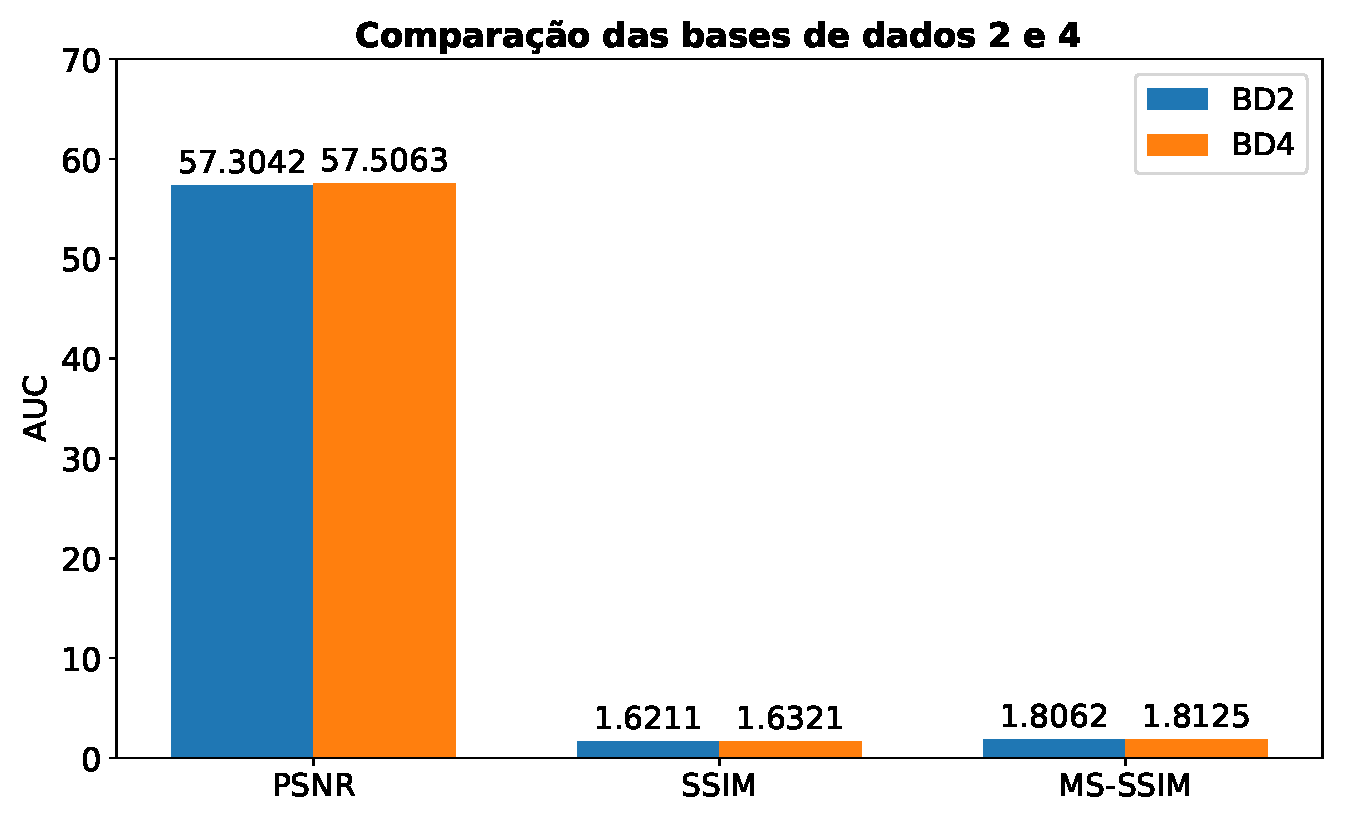
\includegraphics[width=0.7\textwidth]{figuras/auc1.pdf}
%	\caption[Comparação dos resultados das bases de dados 2 e 4.]{Essa Figura mostra resultados das áreas abaixo da curvas de \acrshort{psnr}, \acrshort{ssim} e \acrshort{msssim} em função das taxas nominais, usando os modelos treinados por DB2 e DB4.}
%	\label{fig:auc1}
%\end{figure}

%A BD4 obteve os melhores resultados nas 3 métricas nesse conjunto de teste e será %aplicada nas próximas análises.

\section{Treinamentos em Muitas Épocas}
O próximo passo foi analisar o desempenho no modelo à medida que aumentarmos o número de épocas de treinamento.


Treinamos a rede por 13 épocas usando a base de dados 4. Os parâmetros do novo treinamento foram definidos conforme itens citados em \ref{enum:hiper_param}, exceto o número de épocas. A evolução do modelo ao passar das épocas pode ser vista na Figura \ref{fig:psnr_13epocas}. 

\begin{figure}
	\centering
	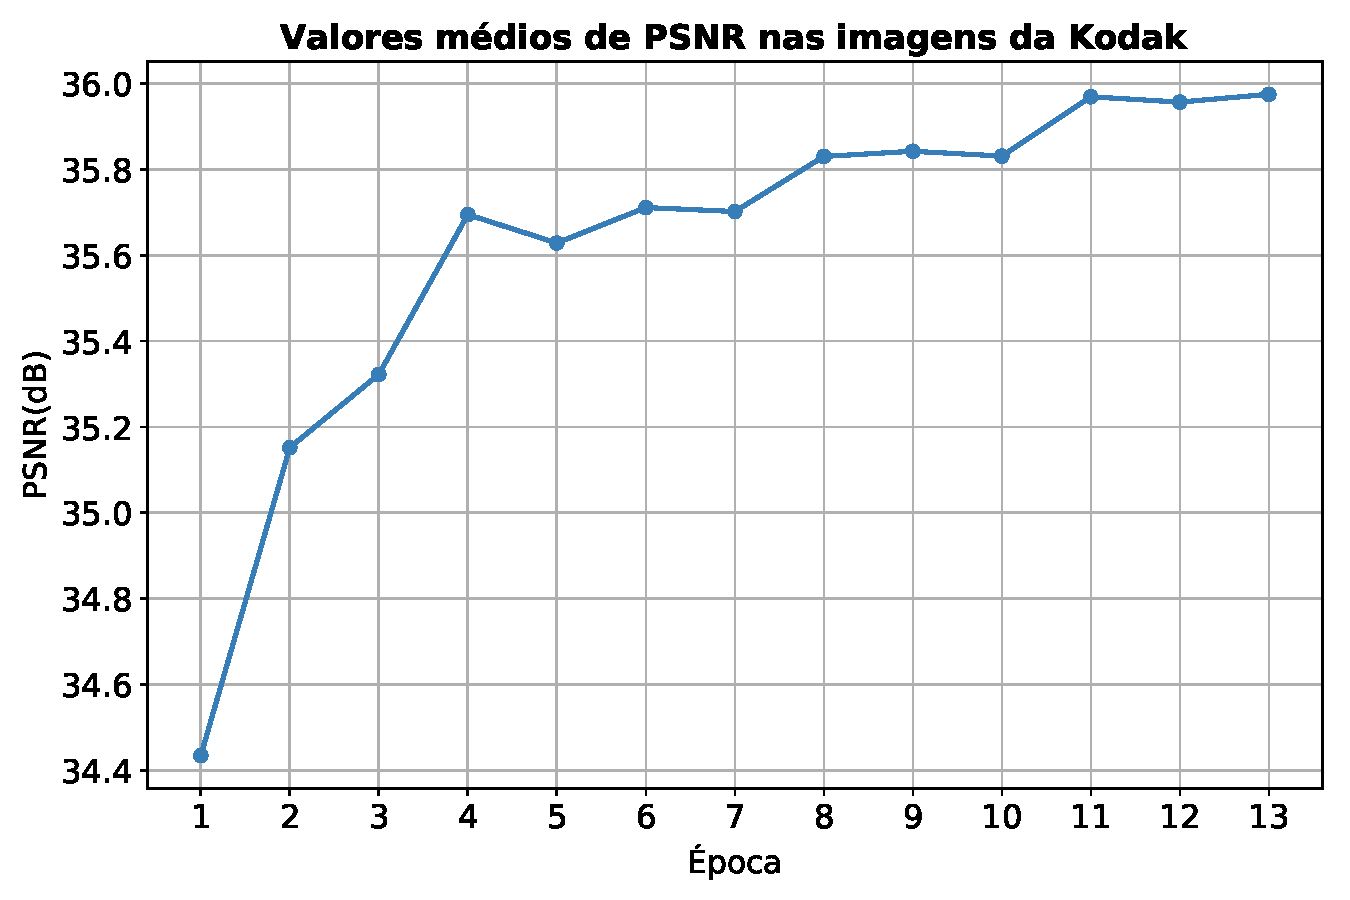
\includegraphics[width=0.9\textwidth]{figuras/psnr_13epochs.pdf}
	\caption[Performance do modelo em função do número de épocas de treinamento]{Performance do modelo em função do número de épocas de treinamento. Para cada época, calculamos a \acrshort{psnr} média das imagens da Kodak reconstruídas com taxa de 2 bpp.  O ganho de desempenho do autocodificador entre a primeira e 13ª época foi de um pouco mais que 1,5dB.}
	\label{fig:psnr_13epocas}
\end{figure}		

Usando o modelo obtido na 13ª época, plotamos as curvas de distorção nas métricas \acrshort{ssim} e \acrshort{msssim} em conjunto com o \acrshort{jpeg}(4:2:0) e o trabalho de Toderici et. al. \cite{FullResolution2017Toderici}. Essas Figuras estão disponíveis em \ref{fig:ssim_ae_jpeg_toderici} e  \ref{fig:msssim_ae_jpeg_toderici}. 
Nessas métricas e na média das imagens da Kodak, nosso modelo supera o trabalho \cite{FullResolution2017Toderici} e o \acrshort{jpeg}. Acreditamos que esse resultado se deve a metodologia para a obtenção da base de dados de treinamento, proposta em \cite{DeliverableJuly}, e duas mudanças propostas na arquitetura original. Essas alterações incluem o processo de treinamento da rede, ao empregarmos a equação \ref{eq:model_1it} ao invés de \ref{eq:ae_full}, e a utilização da \acrshort{mae} ao invés da norma \textit{$L_1$} como função de custo.  


Todavia, a Figura \ref{fig:psnr_ae_jpeg} indica que na métrica \acrshort{psnr} o \acrshort{jpeg}(4:2:0) supera o nosso modelo para a maioria das taxas calculadas. 
%Pela Figura \ref{fig:psnr_13epocas} verificamos uma tendência de saturação do modelo, em torno de 36 dB na taxa de 2 bpp, ao passar das épocas de treinamento. 

% que não passaram por processos de compressão com perdas e decimação.
\begin{figure}
	\centering
	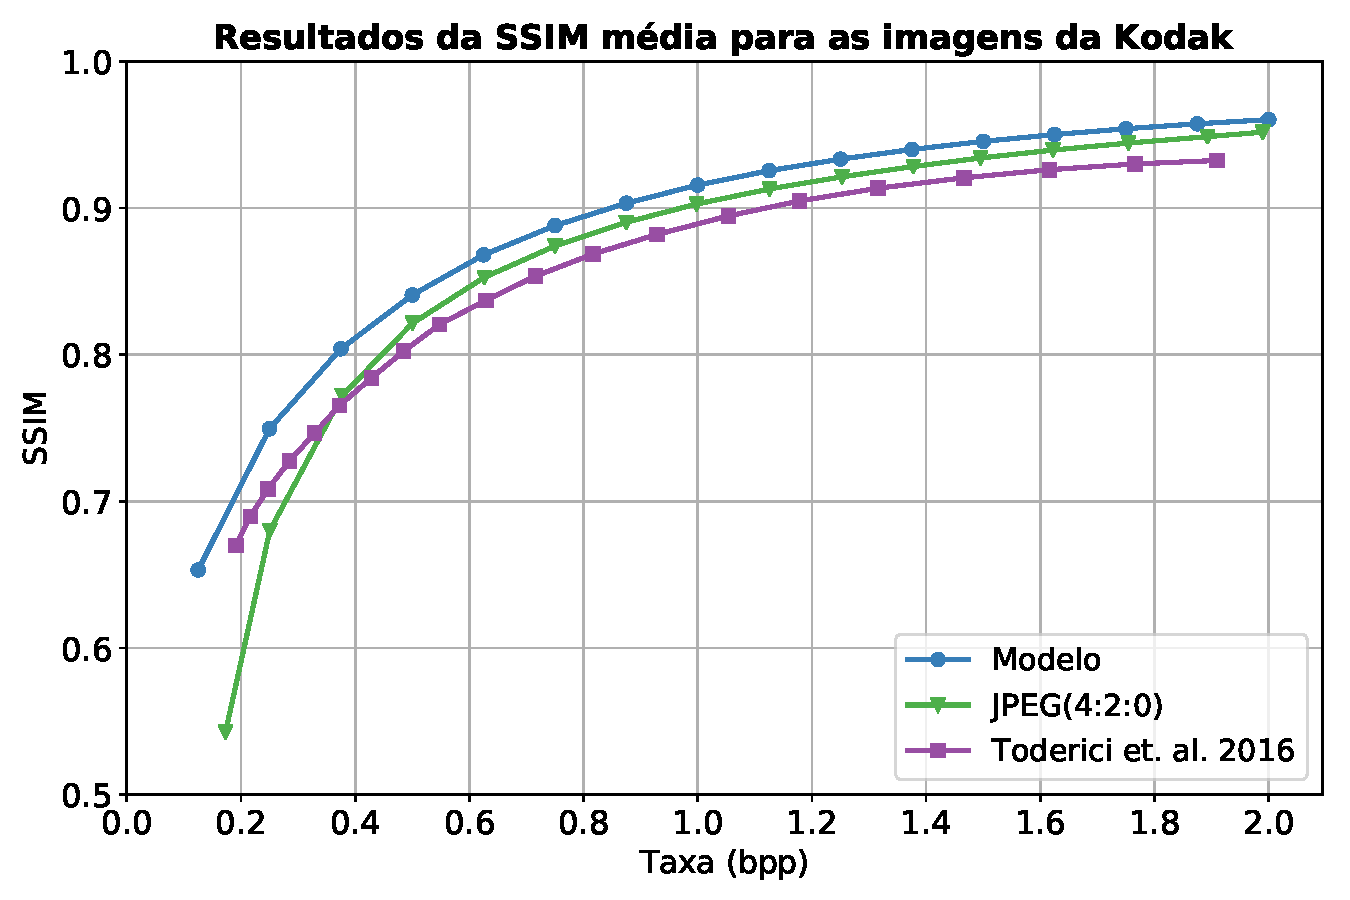
\includegraphics[width=0.9\textwidth]{figuras/ssim_ae_jpeg_toderici.pdf}
	\caption[Curva \acrshort{ssim} por Taxa.]{Desempenho do modelo treinado em 16 épocas e otimizado por \acrshort{mae} em \acrshort{ssim}. Nas taxas apresentadas, obtemos melhores resultados em relação ao \acrshort{jpeg} e o trabalho de Toderici et al. \cite{FullResolution2017Toderici}.}
	\label{fig:ssim_ae_jpeg_toderici}
\end{figure}	


\begin{figure}
	\centering
	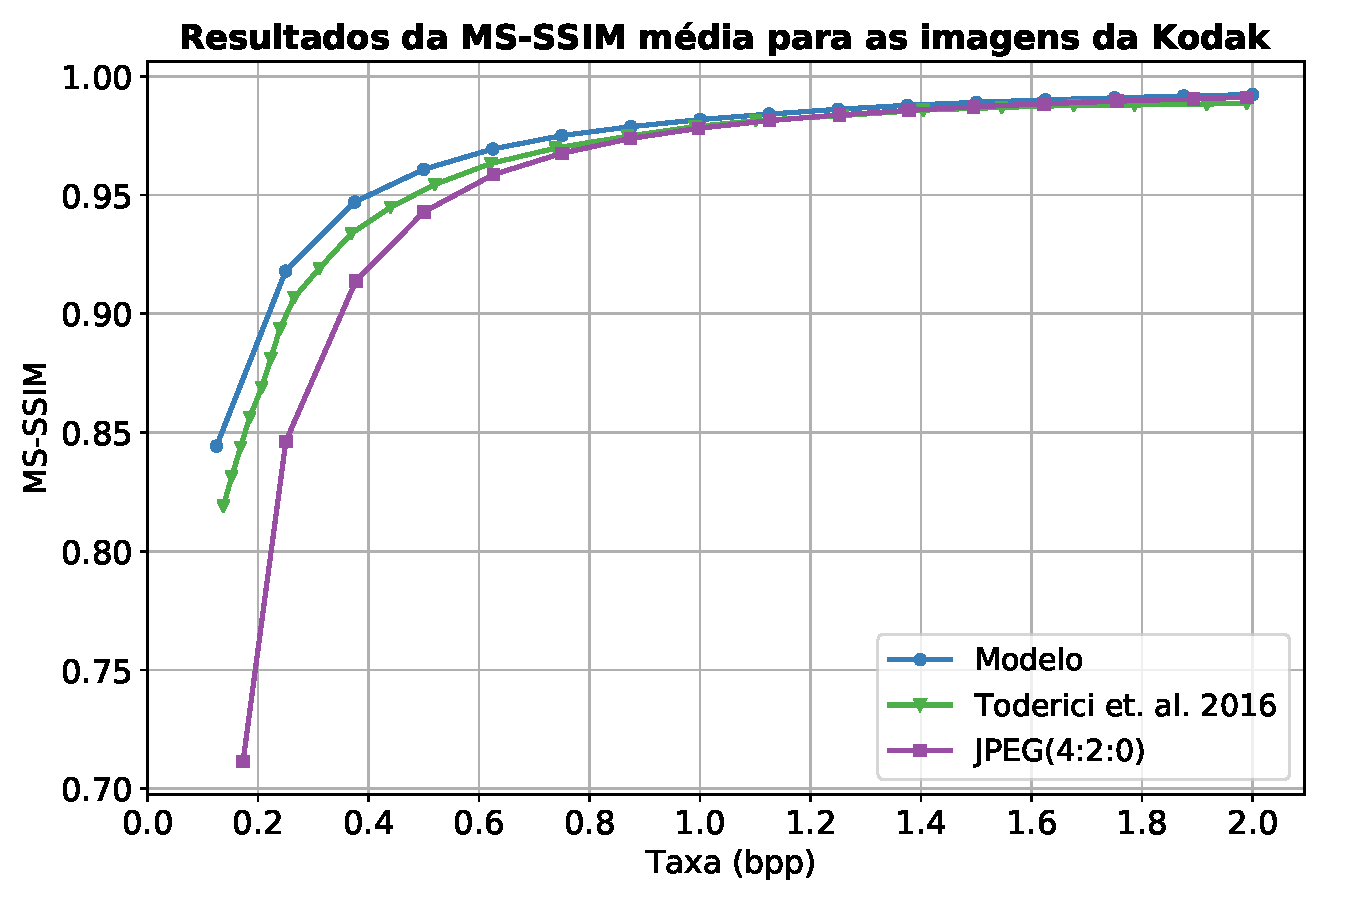
\includegraphics[width=0.9\textwidth]{figuras/msssim_ae_jpeg_toderici.pdf}
	\caption[Curva \acrshort{msssim} por Taxa.]{Comparação do modelo, treinado em 16 épocas e otimizado por \acrshort{mae}, com o \acrshort{jpeg} e o trabalho de Toderici et al. \cite{FullResolution2017Toderici}.}
	\label{fig:msssim_ae_jpeg_toderici}
\end{figure}	



\begin{figure}
	\centering
	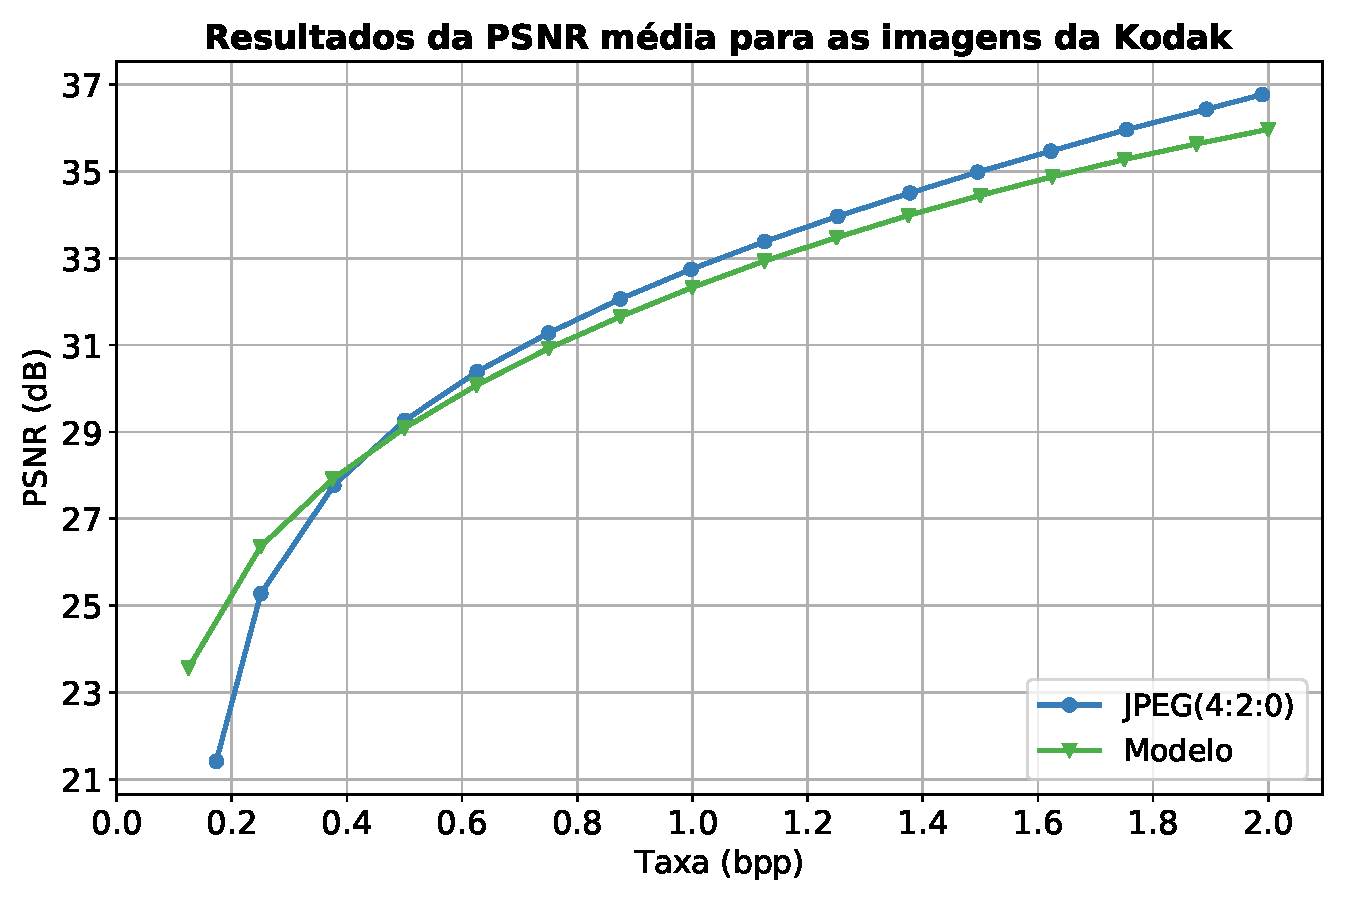
\includegraphics[width=0.9\textwidth]{figuras/psnr_ae_jpeg.pdf}
	\caption[Curva \acrshort{psnr} por Taxa]{Comparação do modelo treinado por 16 épocas com o \acrshort{jpeg}. O modelo supera o \acrshort{jpeg} em \acrshort{psnr} apenas em baixas taxas.}
	\label{fig:psnr_ae_jpeg}
\end{figure}	



%Dessa forma, exploraremos novas técnicas que podem gerar menores taxas de compressão sem impactar na qualidade das imagens reconstruídas pelo decodificador.


%A função de custo é outra escolha importante nos treinamentos de RNA. No problema de compressão de imagens a escolha dessa função tem o agravante de não haver consenso entre os pesquisadores de uma métrica ideal para avaliar a qualidade entre uma imagem original e a sua versão reconstruída.  Na hipótese de haver tal função, poderíamos definir uma função de erro em relação a métrica ideal como função de custo e minimizar o seu valor ao longo do aprendizado do modelo. 
%Contudo, algumas funções apresentam relações da medida de distorção entre uma imagem e sua reconstrução, tais como \acrshort{mse}, \acrshort{mae}, 1-SSIM, 1-MS-SSIM, etc. Vamos definir algumas variações dessas funções. 


%\begin{equation}
%	\begin{aligned}
%    \centering    
%      \acrshort{mae}(X,X') = \displaystyle\frac{1}{n}\sum_{t=1}^{n}\left\|X_{t} - X'_{t}\right\|
%	\end{aligned}
%\end{equation}


\section{Função de Custo}

Esta seção apresenta os testes realizados para diferentes funções de custos para medir a distorção entre imagens. Também analisamos dois método para calcular a informação residual, citados em \ref{sec:arq}.    


A Tabela \ref{table:comp_loss} apresenta resultados para 7 funções de custo relacionadas a distorção entre duas imagens.  Os valores foram calculados pela média das imagens da Kodak, codificadas a 2 bpp. A rede foi treinada com a base de dados 4 e parâmetros listados em \ref{enum:hiper_param}. Nessa tabela, $R$, $R'$, $X$ e $X'$ foram definidos na Equação \ref{eq:model_1it}, omitindo-se a dependência temporal. A medida $X-X'$ é o resíduo em relação à imagem original $X$.  
O subíndice \textit{y} e \textit{$C_bC_r$} são para indicar a componente de luminância e o par crominância azul e vermelho, respectivamente. Nos testes 3 e 4, modificamos o treinamento para rede operar no espaço $YC_bC_r$. O objetivo foi penalizar, predominante, o erro da componente de luminância (que contém informações mais sensíveis ao olho humano) no ajuste da rede, em comparação com as componentes de crominância.
No teste 7, utilizamos uma medida de dissimilaridade estrutural entre duas imagens, obtida a partir da \acrshort{ssim} e implementada em \cite{su2017}.  A distorção calculada pela \acrshort{mse} aplicada no resíduos de reconstruções a nível de iteração ($R-R'$) forneceu os melhores resultados em todas as métricas avaliadas. 


\begin{table}[]
	\centering
	\caption{Comparação das funções de custo.}
	\scalebox{0.9}{
		\begin{tabular}{|c|c|c|c|c|c|c|}
			\hline
			\textbf{Teste} & \textbf{Função de custo}                                                                                        & \textbf{Espaco} & \textbf{PNSR (dB)} & \textbf{PNSR Y (dB)} & \textbf{SSIM}   & \textbf{MS-SIM} \\ \hline
			1     & $MAE(R-R’)$                                                                                                     & RGB             & 33,0872            & 33,8443              & 0,9309          & 0,9876          \\ \hline
			2     & $MAE^{2}(R-R’)$                                                                                                 & RGB             & 34,1766            & 34,9706              & 0,9444          & 0,9892          \\ \hline
			3     & \begin{tabular}[c]{@{}l@{}}$MAE^{2}(R_{y}-R_{y}’) +$\\ $+ 0.25 \times \acrshort{mae}^{2}(R_{CbCr}-R_{CbCr}’)$\end{tabular} & YCbCr           & 33,3555            & 35,3253              & 0,9445          & 0,9857          \\ \hline
			4     & \begin{tabular}[c]{@{}l@{}}$MSE(R_{y}-R_{y}’) +$\\ $+ 0.25 \times \acrshort{mse}(R_{CbCr}-R_{CbCr}’)$\end{tabular}         & YCbCr           & 33,5249            & 35,1863              & 0,9390          & 0,9858          \\ \hline
			\textbf{5}     & $MSE(R-R’)$                                                                                                     & RGB             & \textbf{34,9259}   & \textbf{35,9066}     & \textbf{0,9474} & \textbf{0,9907} \\ \hline
			6     & $MSE(X-X’)$                                                                                                     & RGB             & 33,7662            & 34,6014              & 0,9321          & 0,9866          \\ \hline
			7     & $1 - \acrshort{ssim} (X -X’)$                                                                                              & RGB             & 33,2754            & 34,0755              & 0,9352          & 0,9896          \\ \hline
	\end{tabular}}
	\label{table:comp_loss}
\end{table}

A segunda etapa na escolha de uma função de perdas foi considerar, de forma implícita, a taxa de bits ao aplicar a função \ref{eq:rdo} com $\lambda(t)$ obtido de forma experimental e dado por: 

\begin{equation}
\lambda(t) = 3,5 \times 10^{-7} \times e^{-0,1 \times (t+1)}  
\end{equation}

Para o treinamento usamos a base de dados 5 e alteramos o número de estágios de 16 para 28. Esse aumento visa obter imagens mais precisas pela adição de novos resíduos. Acreditamos que o aumento da taxa nominal seja compensado pela codificação com o GZIP. No novo treinamento da rede teremos:

\begin{enumerate}
	\label{enum:hiper_param2}
	\item Tamanho do lote: 32;  
	\item Número de lotes de treinamento por época: 71 mil (aproximadamente);   
	\item Número de iterações no treinamento: 28;
	\item Número de iterações durante os testes: 22;
	\item Número de épocas: 27;
	\item Taxa de aprendizado: $5 \times {10}^{-4}$ com decaimento por um fator de 0,5 caso a média da função de custo em uma época seja maior que na época anterior.
\end{enumerate}


\section{Análise da Codificação de Entropia para o Desempenho do Autocodificador Recorrente e Esparso}

Esta seção aborda os resultados do modelo baseados em esparsidade do código binário. Medimos a eficiência dessa abordagem pela redução das taxas nominais usando a codificação de entropia fornecida pelo GZIP, e pela distorção das imagens obtida após a compressão. A otimização de distorção e, implicitamente, de taxa é, possivelmente, a principal contribuição deste trabalho.    


A Figura \ref{fig:gain_gzip_meida} apresenta resultados após a codificação de entropia do GZIP. As curvas de \acrshort{psnr} e \acrshort{ssim} se deslocam para esquerda em virtude de taxas reais serem menores que as nominais. O ganho do GZIP é maior para altas taxas. Isso é esperado tendo em vista que, em geral, os codificadores de entropia são mais eficientes em conjuntos maiores de dados. Nos próximos testes, as taxas empregadas serão sempre a real.    

\begin{figure}
	\centering
	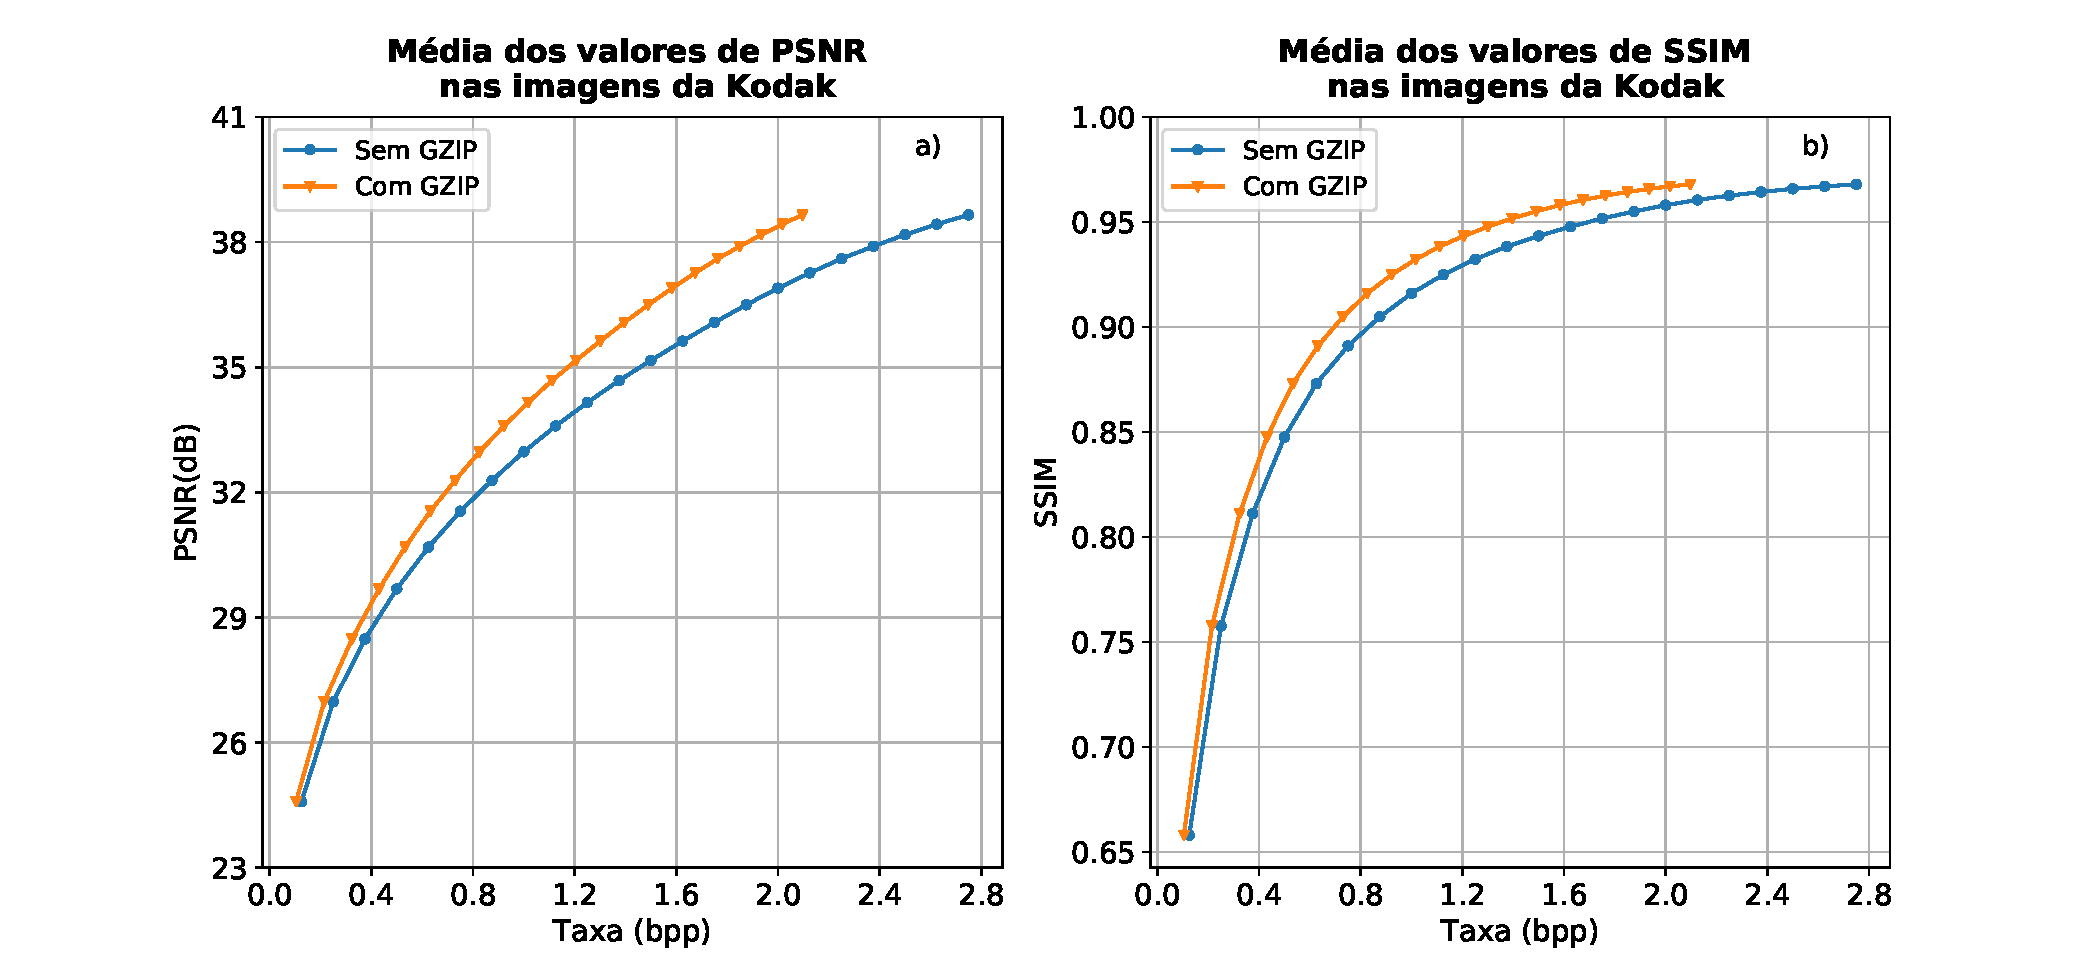
\includegraphics[width=1.1\textwidth]{figuras/gain_gzip_media.pdf}
	\caption[Curvas antes e após codificação com o GZIP]{Nessa figura, ilustramos o resultado em aplicar o GZIP na sequência binária gerada no codificador. As curvas foram plotadas usando o modelo treinado até a época 26.}  	
	\label{fig:gain_gzip_meida}
\end{figure}

A Figura \ref{fig:taxa_bd} mostra como o desempenho, em termos de \acrshort{bdrate}, (em relação ao \acrshort{jpeg}) se comporta durante o treinamento do modelo. O treinamento em várias épocas melhora, significativamente, o seu desempenho, como visto anteriormente. É verdade também que a velocidade na qual o modelo apresenta melhores resultados reduz ao passar das épocas. A economia do \acrshort{codec} na 26ª época em relação à primeira é de, aproximadamente, 17\%. A arquitetura treinada até a 26ª época possui os melhores resultados. 


\begin{figure}
	\centering
	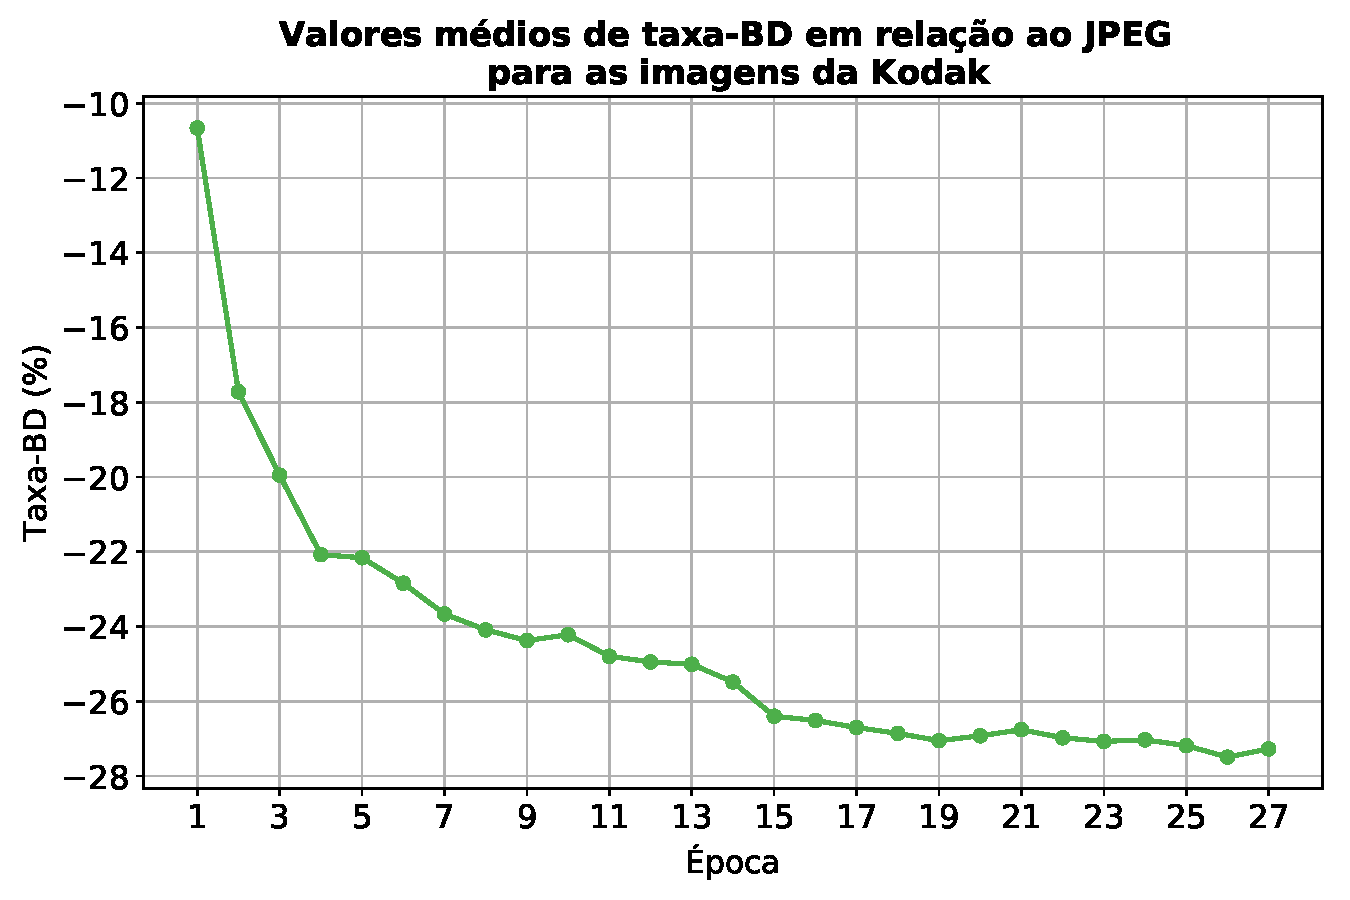
\includegraphics[width=1\textwidth]{figuras/taxa_bd_27epocas.pdf}
	\caption[Curva de \acrshort{bdrate} por época de treinamento.]{Ilustração da porcentagem da \acrshort{bdrate} média sobre a base de dados da Kodak e tendo o \acrshort{jpeg} como âncora.  Valores cada vez mais negativos indicam que a economia média de taxa de bits do nosso modelo em relação ao \acrshort{jpeg} aumenta para uma dada qualidade equivalente de \acrshort{psnr} na média das imagens da Kodak.}  
	\label{fig:taxa_bd}
\end{figure}	

Nas Figuras em \ref{fig:metricas_3ep} podemos observar a otimização em 3 épocas através de curvas taxa-distorção. Nesse teste, a qualidade melhora e a taxa real é reduzida seguindo a época 1, 6 e 26. A qualidade aqui é dada pelas curvas de \acrshort{psnr} (a), \acrshort{psnr} Y (b)  \acrshort{ssim} (c) e  \acrshort{msssim} (d). Esses resultados mostram que a nossa função realiza uma otimização conjunta de distorção e taxa. 
%Todavia, não temos uma fundamentação na direção do melhor método para otimização taxa-distorção.  

\begin{figure}
	\centering
	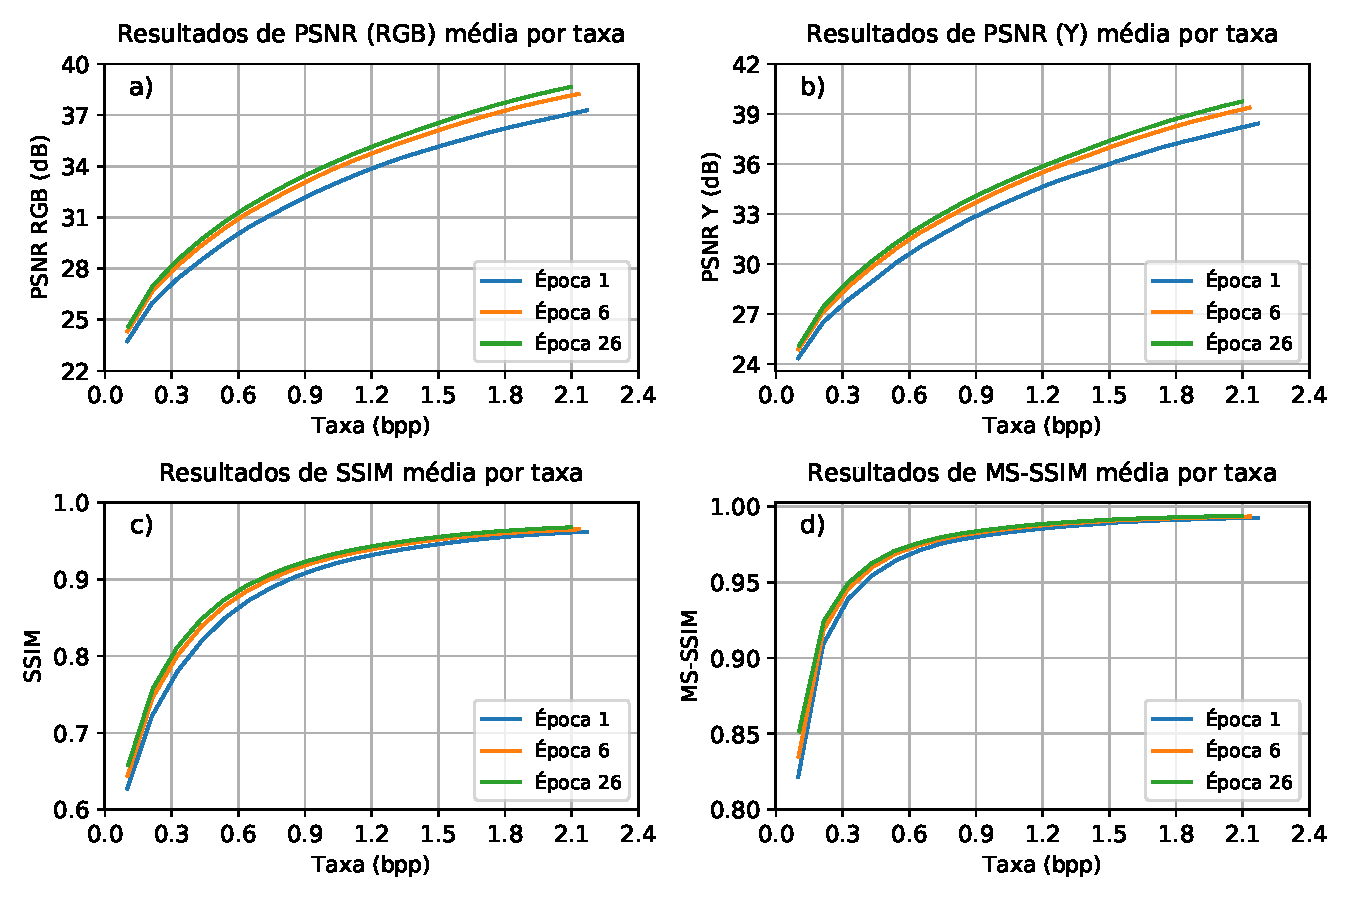
\includegraphics[width=1\textwidth]{figuras/result_3ep.pdf}
	\caption[Curvas de qualidade por taxa em 3 épocas distintas]{Figuras mostrando a evolução do modelo em termos de taxa e 4 métricas de qualidade para 3 épocas distintas. Nas 4 curvas taxa e distorção apresentam melhores resultado à medida que o número de épocas aumenta. Taxas reais calculadas. }  	
	\label{fig:metricas_3ep}
\end{figure}

A Figura \ref{fig:gain_medio_bpp} apresenta o ganho médio percentual da taxa real (fornecida pelo GZIP) em relação a nominal, em  função do número de iterações nas quais as imagens foram reconstruídas. Os resultados mostram que nos primeiros 3 níveis de reconstrução o modelo de melhor desempenho (modelo26) tem ganho médio de taxa menor em relação aos modelos com \textit{underfitting}.  


\begin{figure}
	\centering
	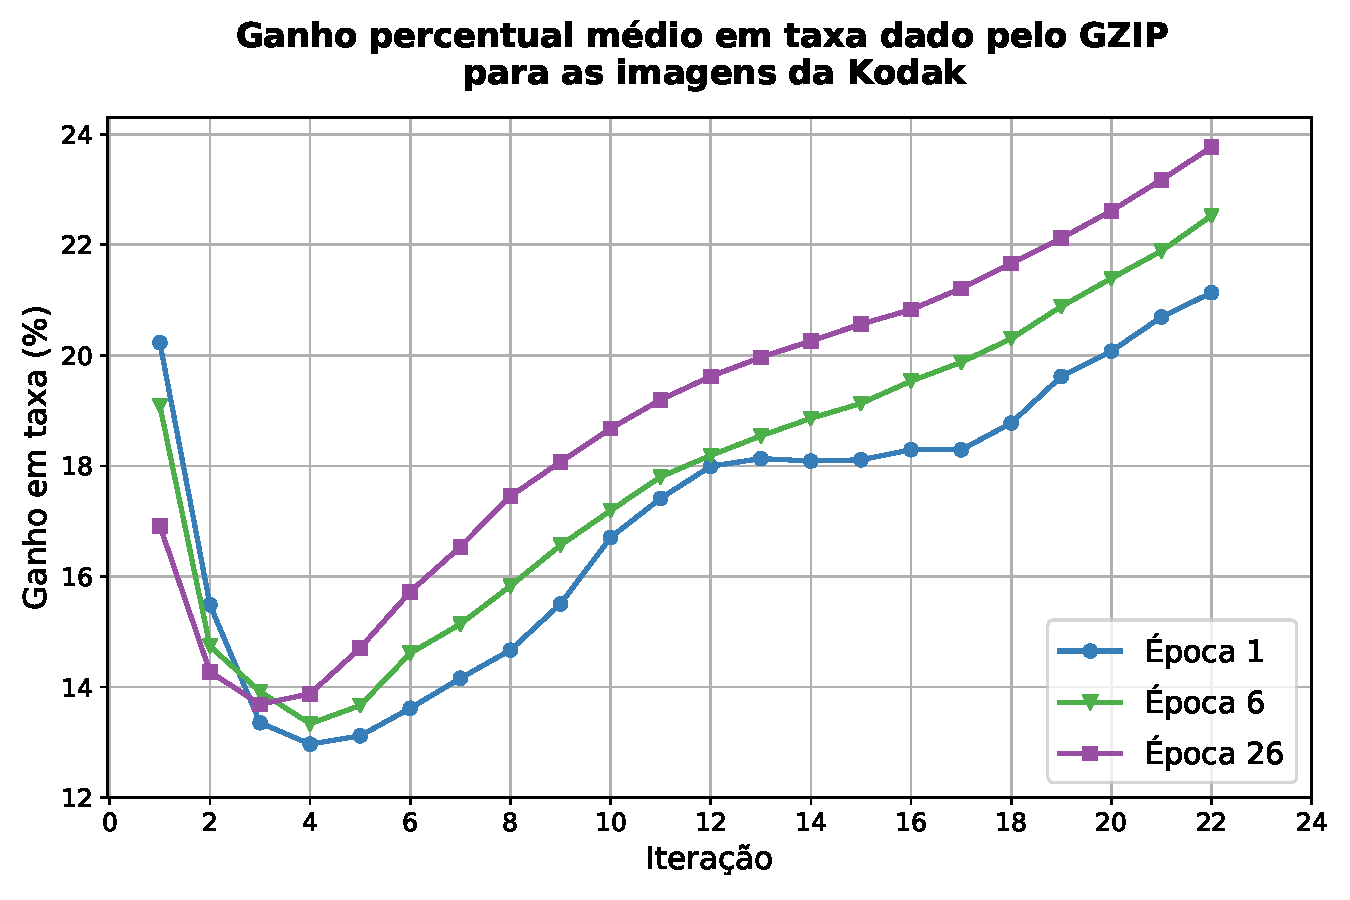
\includegraphics[width=0.9\textwidth]{figuras/ganho_taxa_3epocas.pdf}
	\caption[Ganho do GZIP por nível de reconstrução]{Ganho do GZIP por nível de reconstrução para 3 modelos. Nas primeiras iterações o ganho é progressivamente menor e a partir da quarta iteração o ganho de taxa é crescente (aproximadamente).}  	
	\label{fig:gain_medio_bpp}
\end{figure}

%, ainda que temos um conjunto maior de bits para realizar compressão.

A justificativa pode ser que durante o treinamento, para esse nível de reconstrução a função da distorção é significativamente superior ao valor da função de esparsidade. Ao priorizar a reconstrução o código binário deve apresentar menor redundância. Isso implica em menor margem para a redução das taxas nominais após codificação de entropia. 
A partir da 4ª iteração a curva de ganho do modelo final ultrapassa as demais. Acreditamos que, conforme a reconstrução é feita, a relevância da distorção medida pela \acrshort{mse} sofra redução e consequentemente a função de esparsidade reduza, consideravelmente, a entropia de primeira ordem do código binário. Vamos usar o modelo de melhor ajuste (modelo26) para realizar as próximas análises.  

A Tabela em \ref{table:entrop} apresenta quantidades percentuais de bits 1 e 0 no fluxo de bits por nível de iteração e na média das imagens da Kodak. A cada iteração 49152 bits são adicionados ao fluxo de dados enviados ao decodificador. 
É interessante observar como o modelo penaliza a ocorrência do bit de valor 1. À medida que reconstruímos uma imagem e montamos o fluxo de bits, menor é a porcentagem de ocorrência desse bit.  Portanto, a entropia de primeira ordem é um função decrescente do número de iterações, conforme apresentado na quinta coluna dessa tabela.  A nossa  abordagem foi eficaz para promover esparsidade no código binário. 
Fato a destacar é que nas primeiras 3 iterações na Figura \ref{fig:gain_medio_bpp} o ganho de taxa é sucessivamente menor, contudo nesse mesmo intervalo a proporção de bits 0 é progressivamente menor.  Ou seja, ainda que nossa função de custo esteja promovendo esparsidade (e reduzindo a entropia de primeira ordem) isso não significou, nesse intervalo, que a codificação de entropia seja mais eficiente.  
Logo, a redução na entropia de primeira ordem não implica, necessariamente, em uma codificação de entropia mais eficiente através do GZIP. 


%Logo, faz se necessário um estudo mais fundamentado para modelar  a entropia do código binário e obtemos melhores estimativas da entropia real da fonte. 
%e a eficácia de codificação de entropia. 
%Logo,  redução na entropia de primeira ordem não significa, necessariamente, em uma %codificação de entropia mais eficiente. 


\begin{table}[]
	\centering
	\caption{Estatística do fluxo de bits na compressão das imagens de teste}
	\scalebox{0.9}{
		\begin{tabular}{ccccc}
			\hline
			\textbf{Iteração} & \textbf{\begin{tabular}[c]{@{}c@{}}Quantidade \\ de Bits\end{tabular}} & \textbf{\begin{tabular}[c]{@{}c@{}}Quantidade de\\ Bits 1  (\%)\end{tabular}} & \textbf{\begin{tabular}[c]{@{}c@{}}Quantidade de \\ Bits 0  (\%)\end{tabular}} & \textbf{Entropia (b/s)} \\ \hline
			1                 & 49152                                                                  & 36,43                                                                        & 63,57                                                                             & 0,946                   \\ \hline
			2                 & 98304                                                                  & 33,50                                                                        & 66,50                                                                             & 0,920                   \\ \hline
			3                 & 147456                                                                 & 32,34                                                                        & 67,66                                                                             & 0,908                   \\ \hline
			4                 & 196608                                                                 & 31,51                                                                        & 68,49                                                                             & 0,899                   \\ \hline
			5                 & 245760                                                                 & 30,64                                                                        & 69,36                                                                             & 0,889                   \\ \hline
			6                 & 294912                                                                 & 29,78                                                                        & 70,22                                                                             & 0,879                   \\ \hline
			7                 & 344064                                                                 & 29,03                                                                        & 70,97                                                                             & 0,869                   \\ \hline
			8                 & 393216                                                                 & 28,35                                                                        & 71,65                                                                             & 0,860                   \\ \hline
			9                 & 442368                                                                 & 27,88                                                                        & 72,12                                                                             & 0,854                   \\ \hline
			10                & 491520                                                                 & 27,42                                                                        & 72,58                                                                             & 0,847                   \\ \hline
			11                & 540672                                                                 & 27,00                                                                        & 73,00                                                                             & 0,842                   \\ \hline
			12                & 589824                                                                 & 26,64                                                                        & 73,36                                                                             & 0,836                   \\ \hline
			13                & 638976                                                                 & 26,35                                                                        & 73,65                                                                             & 0,832                   \\ \hline
			14                & 688128                                                                 & 26,09                                                                        & 73,91                                                                             & 0,828                   \\ \hline
			15                & 737280                                                                 & 25,83                                                                        & 74,17                                                                             & 0,824                   \\ \hline
			16                & 786432                                                                 & 25,60                                                                        & 74,40                                                                             & 0,821                   \\ \hline
			17                & 835584                                                                 & 25,30                                                                        & 74,70                                                                             & 0,816                   \\ \hline
			18                & 884736                                                                 & 25,01                                                                        & 74,99                                                                             & 0,811                   \\ \hline
			19                & 933888                                                                 & 24,71                                                                        & 75,29                                                                             & 0,807                   \\ \hline
			20                & 983040                                                                 & 24,39                                                                        & 75,61                                                                             & 0,801                   \\ \hline
			21                & 1032192                                                                & 24,03                                                                        & 75,97                                                                             & 0,796                   \\ \hline
			22                & 1081344                                                                & 23,66                                                                        & 76,34                                                                             & 0,789                   \\ \hline
	\end{tabular}} \quad
	\label{table:entrop}
\end{table}





%\begin{figure}
%	\centering
%	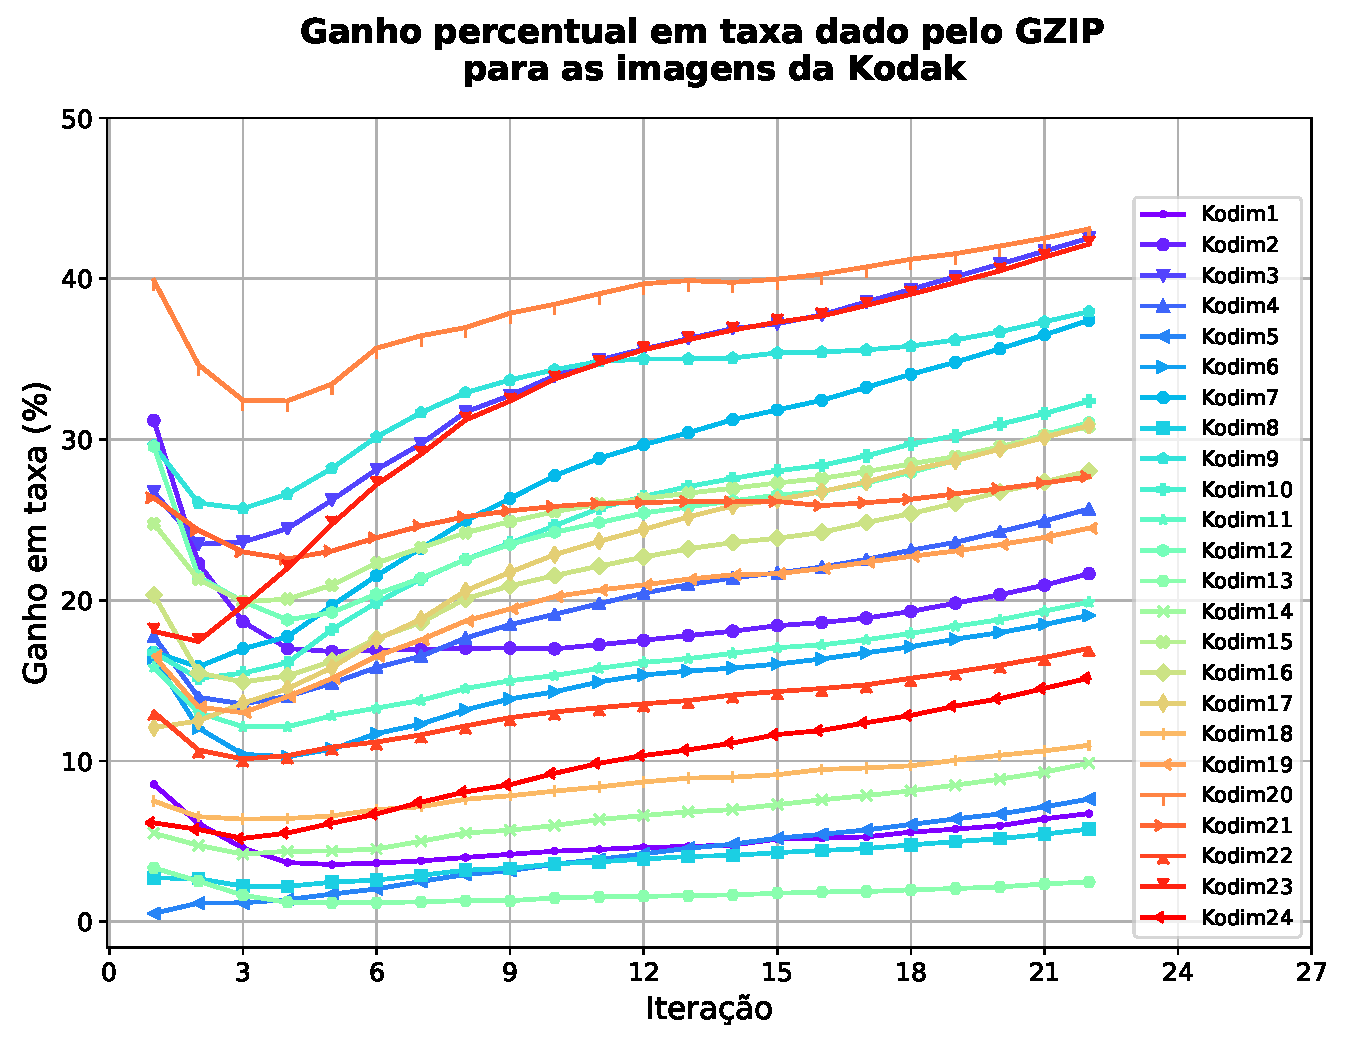
\includegraphics[width=1.0\textwidth]{figuras/ganho_taxa_kodak_epoca26.pdf}
%	\caption{}  	
%	\label{fig:gain_bpp}
%\end{figure}

%\begin{figure}
%	\centering
%	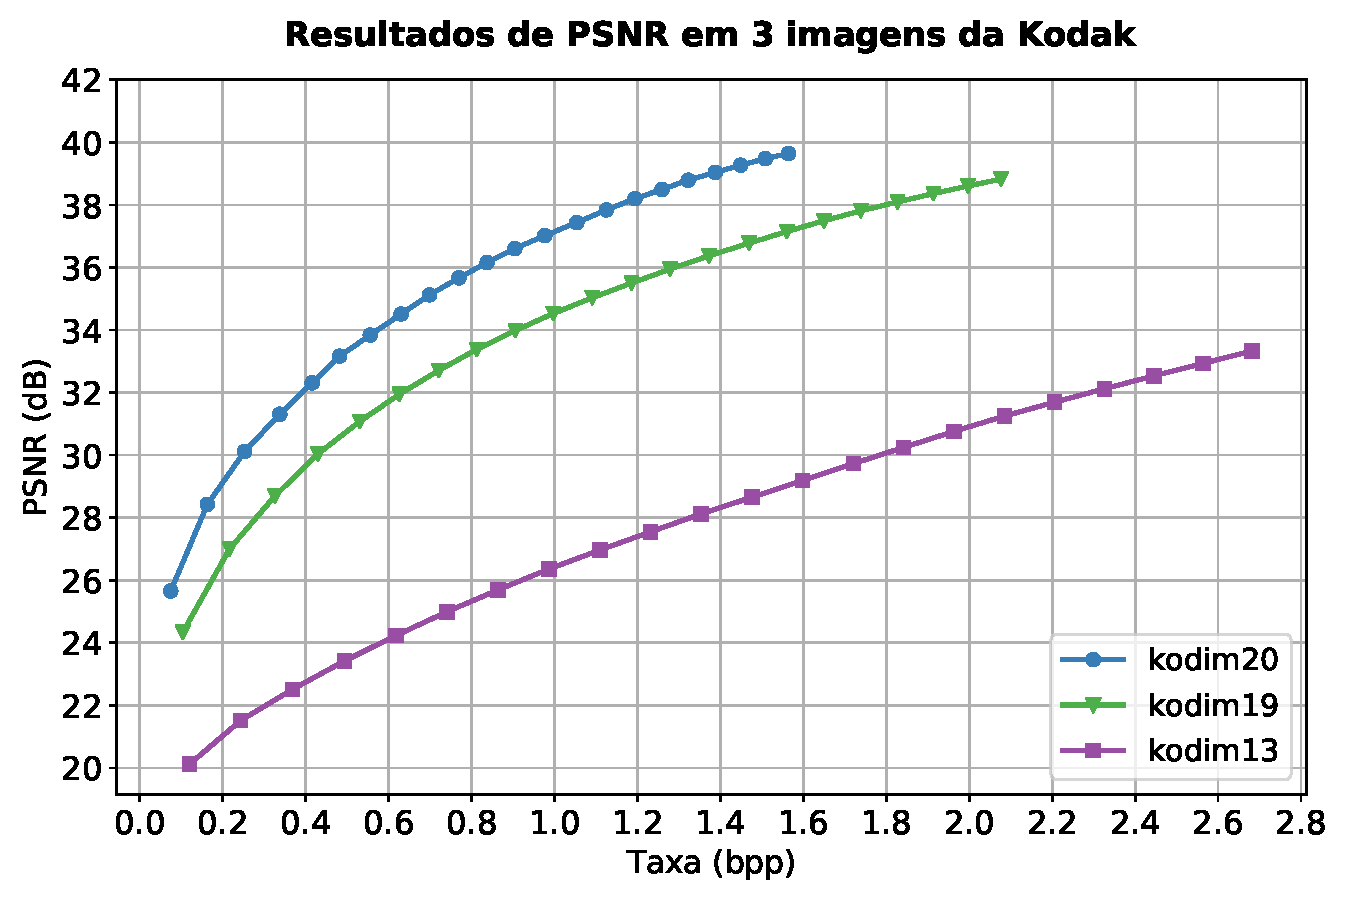
\includegraphics[width=0.9\textwidth]{figuras/rdo_3examples.pdf}
%	\caption{}  	
%	\label{fig:rdo_3examples}
%\end{figure}


Nas Figuras em \ref{fig:comp_gain_psnr} apresentamos 3 curvas de \acrshort{psnr} e ganho dado pelo GZIP. Na base de dado de teste, a imagem 13 da kodak (\textit{kodim13})  obteve o menor ganho, a \textit{kodim20} o maior, e a \textit{kodim6} tem ganho aproximadamente próximo da média. 
Acreditamos que os códigos binários possuem maior redundância nas imagens com conteúdos ``suaves'', (por exemplo céu, mar, etc) como na Figura \ref{fig:kodim20}. 
De forma análoga, imagens com muita informação de alta frequência é de ``difícil compressão'', 
de modo que a estatística dos seus bits não favorece um alto fator de compactação. A \textit{kodim13}, ilustrada na Figura \ref{fig:kodim13}, exemplifica uma imagem com alta taxa de variação da intensidade por \textit{pixel}. 

Uma limitação do nosso modelo é obter altas taxas para algumas imagens mesmo aumentando o número iterações. Por exemplo, na \textit{kodim20}  em relação a uma dada iteração, a qualidade e taxa começam a reduzir à medida que novas iterações são feitas (contra-intuitivamente). A nossa hipótese é que a rede tem dificuldade para reconstruir resíduos com valores pequenos, como foi discutido em \cite{FullResolution2017Toderici}.  Além disso, devido a otimização conjunta de distorção e taxa, provavelmente estamos penalizando excessivamente a frequência de bits 1 em relação a função de distorção. Dessa forma, o modelo gera códigos com baixa entropia, contudo a reconstrução fica prejudicada.   


\begin{figure}
	\centering
	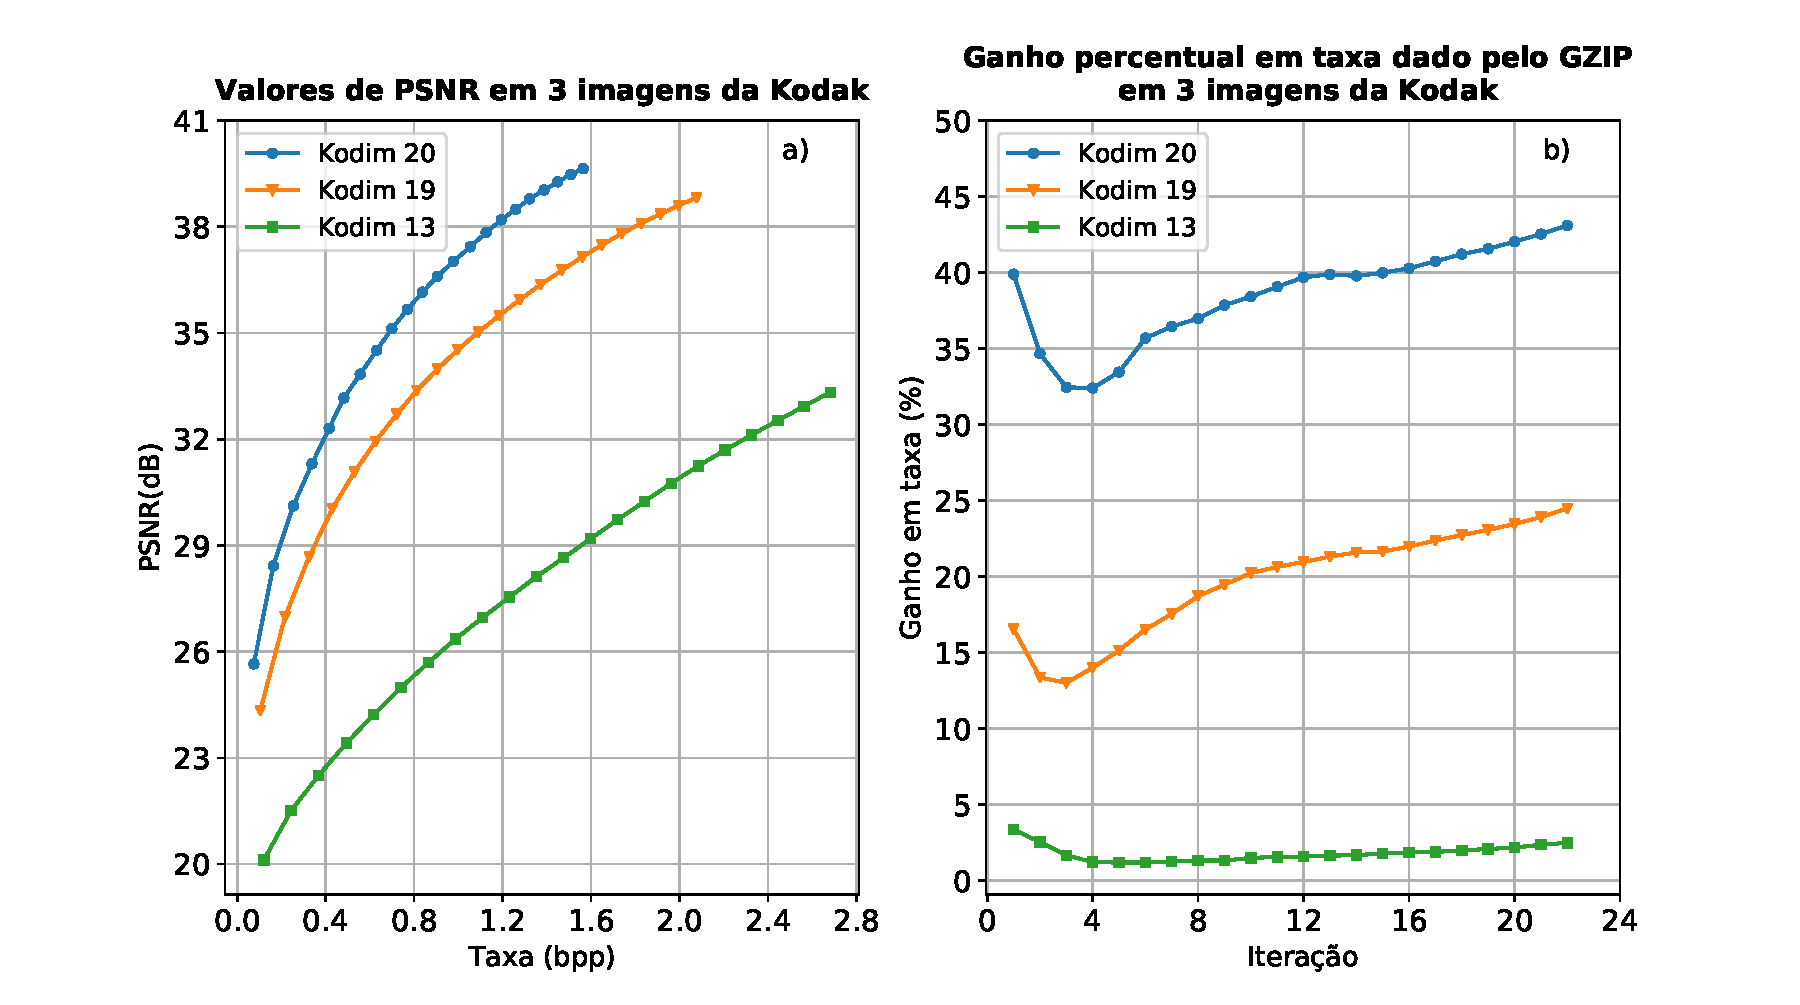
\includegraphics[width=1.0\textwidth]{figuras/comp_gain_psnr.pdf}
	\caption[Comparação em 3 imagens representativas da Kodak.]{Comparação com  3 imagens representativas da base de dados de tese.}   	
	\label{fig:comp_gain_psnr}
\end{figure}

%	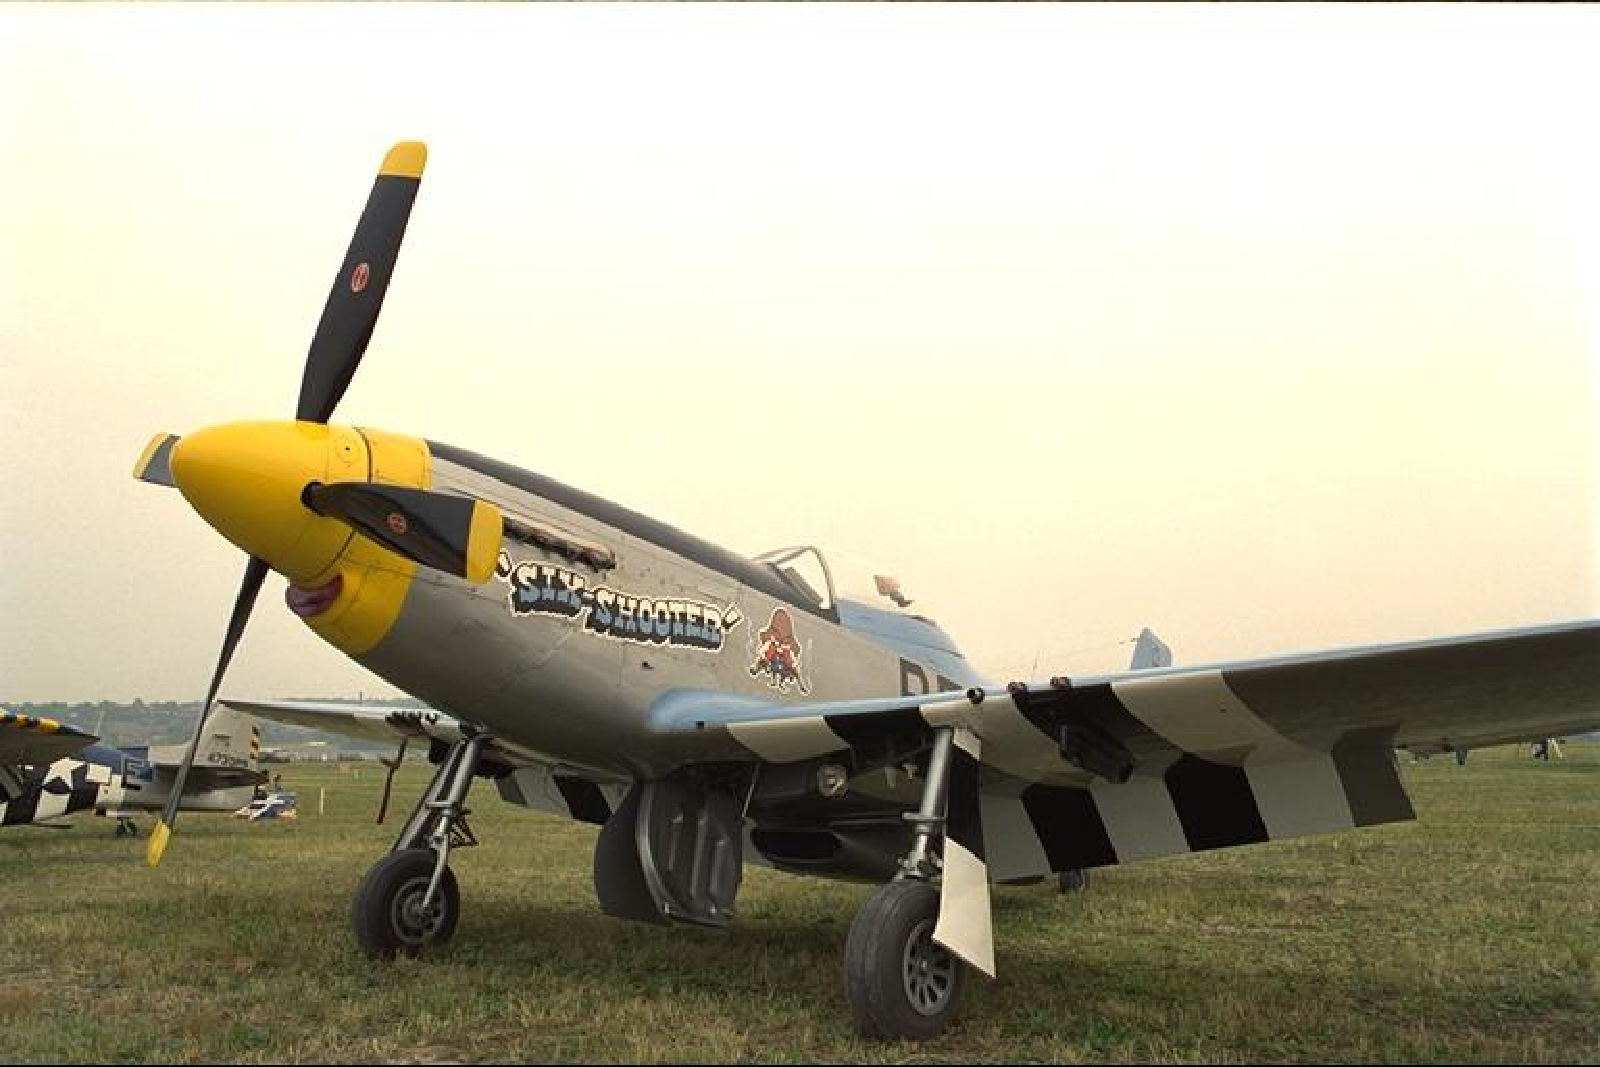
\includegraphics[width=.4\linewidth]{figuras/kodim20}



\begin{figure}
	\subfloat[Imagem original]{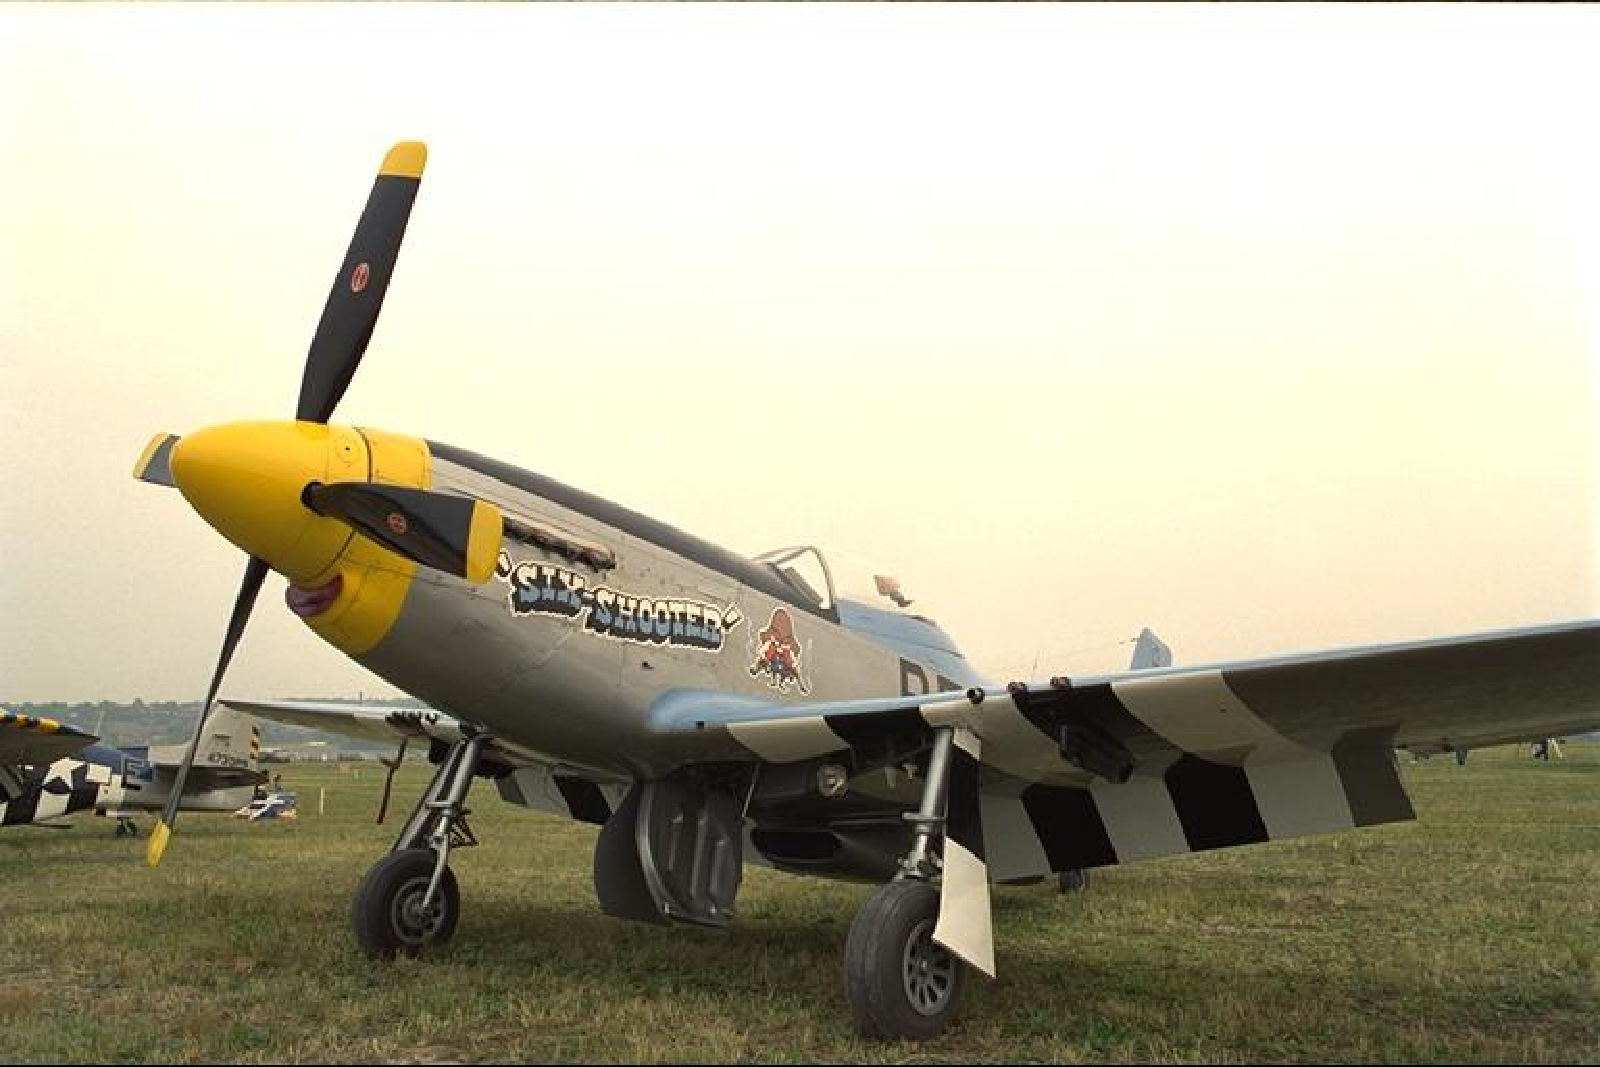
\includegraphics[width=1.0\textwidth]{figuras/kodim20.pdf}}
	\newline
	\subfloat[{Imagem reconstruída. Taxa: 0,942 bpp. \acrshort{psnr}: 36,925 dB.}   ]{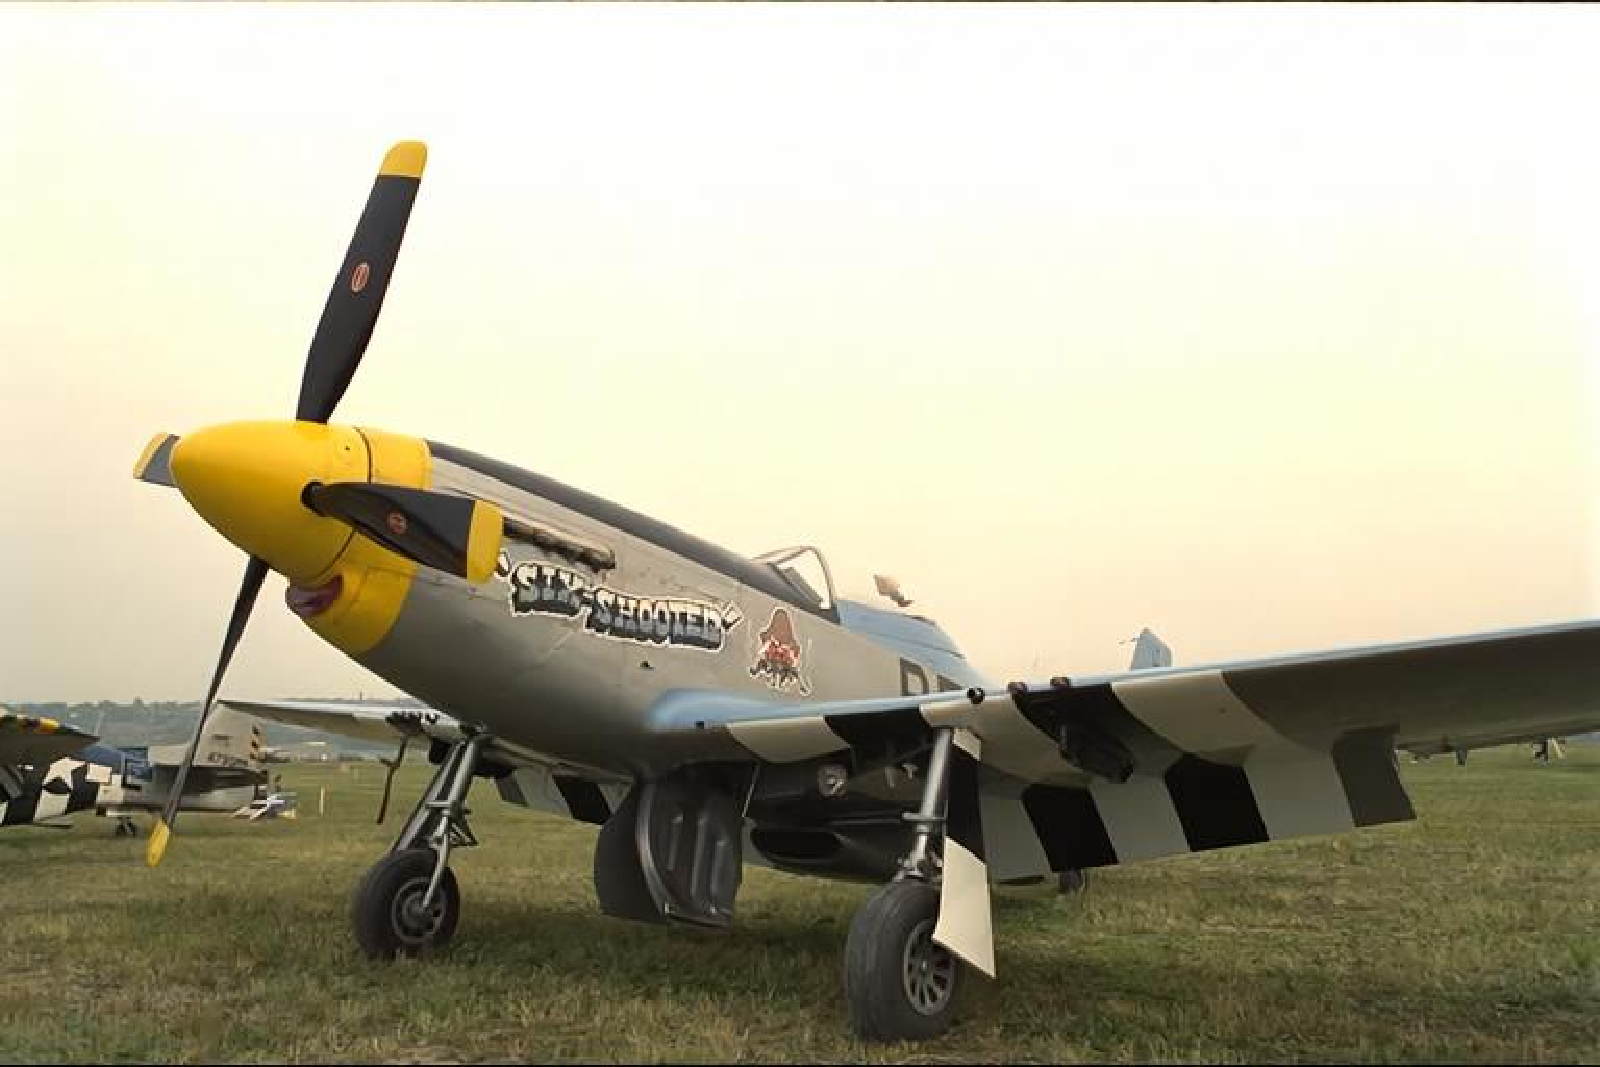
\includegraphics[width=1.0\textwidth]{figuras/kodim20it10.pdf}}
	
	\caption[Imagem representativa com alto fator de compressão]{Em (a) temos a imagem 20 da Kodak (\textit{kodim20}) em (b) sua versão reconstruída em 10 iterações.}
	\label{fig:kodim20}
\end{figure}
\begin{figure}	
	\subfloat[Imagem original]{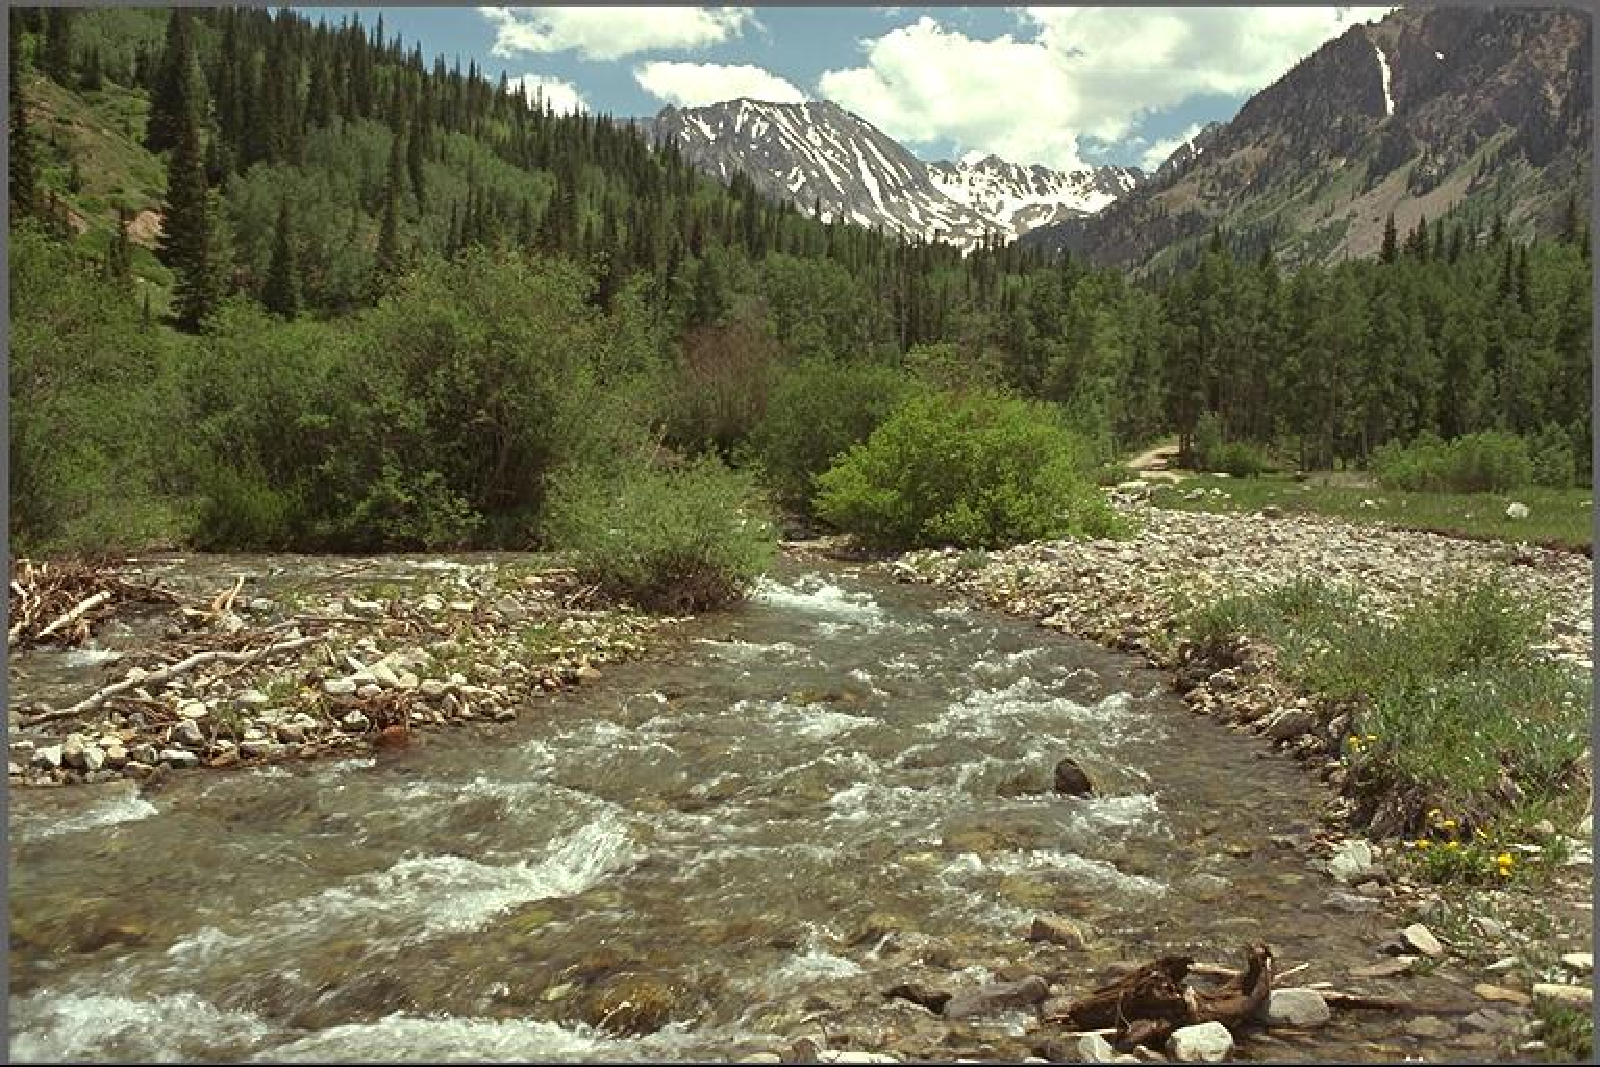
\includegraphics[width=1.0\textwidth]{figuras/kodim13.pdf}}
	\newline
	\subfloat[{Imagem reconstruída. Taxa: 0,987 bpp. \acrshort{psnr}: 26,357 dB.}   ]{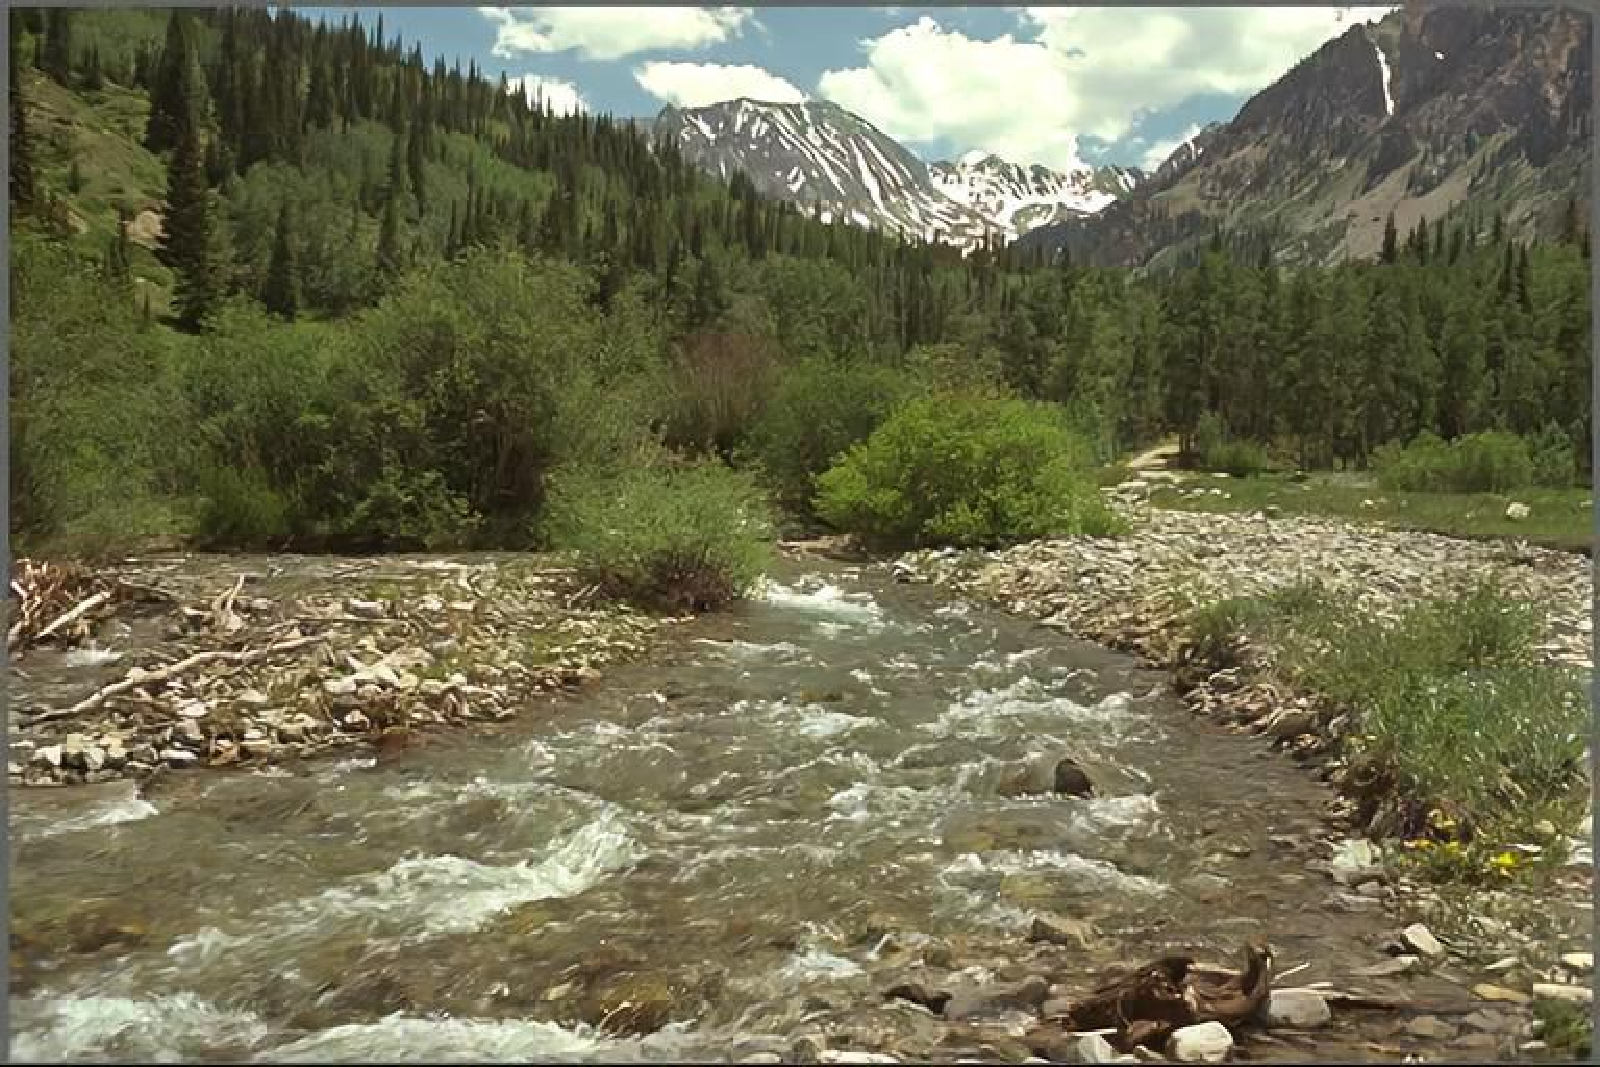
\includegraphics[width=1.0\textwidth]{figuras/kodim13it8.pdf}}
	\caption[Imagem representativa com baixo fator de compressão]{Em (a) está representado a \textit{kodim13} e em (b) sua versão reconstruída em 8 iterações.}
	\label{fig:kodim13}
\end{figure}


\section{Alocação Dinâmica de Bits}

Nessa seção disponibilizamos e discutimos os resultados como o método de alocação dinâmica de bits. 

Definimos dois testes principais para aplicar o método de alocação dinâmica de bits descrito em \ref{sec:adb}. No primeiro, não restringimos o número mínimo de níveis de reconstrução em cada bloco. Isso equivale a fazer $k_{min} = 1$ na Figura \ref{fig:flux_vr}. Referimos  a ele como modeloVR0.  A Tabela \ref{table:ba} apresenta os resultados desse modelo nas imagens da Kodak. Nessa tabela, \acrshort{psnr}$_d$ é o alvo de qualidade desejada e \acrshort{psnr}$_o$ é a qualidade obtida. 



\begin{table}[h]
	\caption{Resultados do Método de Alocação Dinâmica de Bits}
	\centering
	\scalebox{0.9}{
		\begin{tabular}{|c|c|c|}
			
			\hline
			\textbf{PSNR$_d$ (dB)} & \textbf{PSNR$_o$ (dB)} & \textbf{Taxa Real (bpp)} \\ \hline
			24                  & 27,19               & 0,237                    \\ \hline
			25                  & 27,82               & 0,282                    \\ \hline
			26                  & 28,52               & 0,335                    \\ \hline
			27                  & 29,27               & 0,397                    \\ \hline
			28                  & 30,00               & 0,467                    \\ \hline
			29                  & 30,81               & 0,551                    \\ \hline
			30                  & 31,60               & 0,642                    \\ \hline
			31                  & 32,42               & 0,742                    \\ \hline
			32                  & 33,23               & 0,851                    \\ \hline
			33                  & 34,05               & 0,971                    \\ \hline
			34                  & 34,88               & 1,100                    \\ \hline
			35                  & 35,65               & 1,237                    \\ \hline
			36                  & 36,38               & 1,378                    \\ \hline
			37                  & 37,06               & 1,520                    \\ \hline
			38                  & 37,62               & 1,658                    \\ \hline
			39                  & 38,12               & 1,793                    \\ \hline
			40                  & 38,51               & 1,929                    \\ \hline
			41                  & 38,79               & 2,063                    \\ \hline
			42                  & 38,96               & 2,171                    \\ \hline
	\end{tabular}}
	\label{table:ba}
\end{table}


Contudo, tal procedimento gera artefatos de blocos em evidência, como podemos observar na Figura \ref{fig:artefatos1}. 
Então, fazemos $k_{min}=5$ para codificar as imagens pelo modeloVR na tentativa de minimizar o surgimento desses artefatos de compressão. Na figura \ref{fig:artefatos2} há um exemplo de reconstrução com esse modelo e outro sem utilizar a alocação de bits.  


\begin{figure}
	\subfloat[Imagem original.]{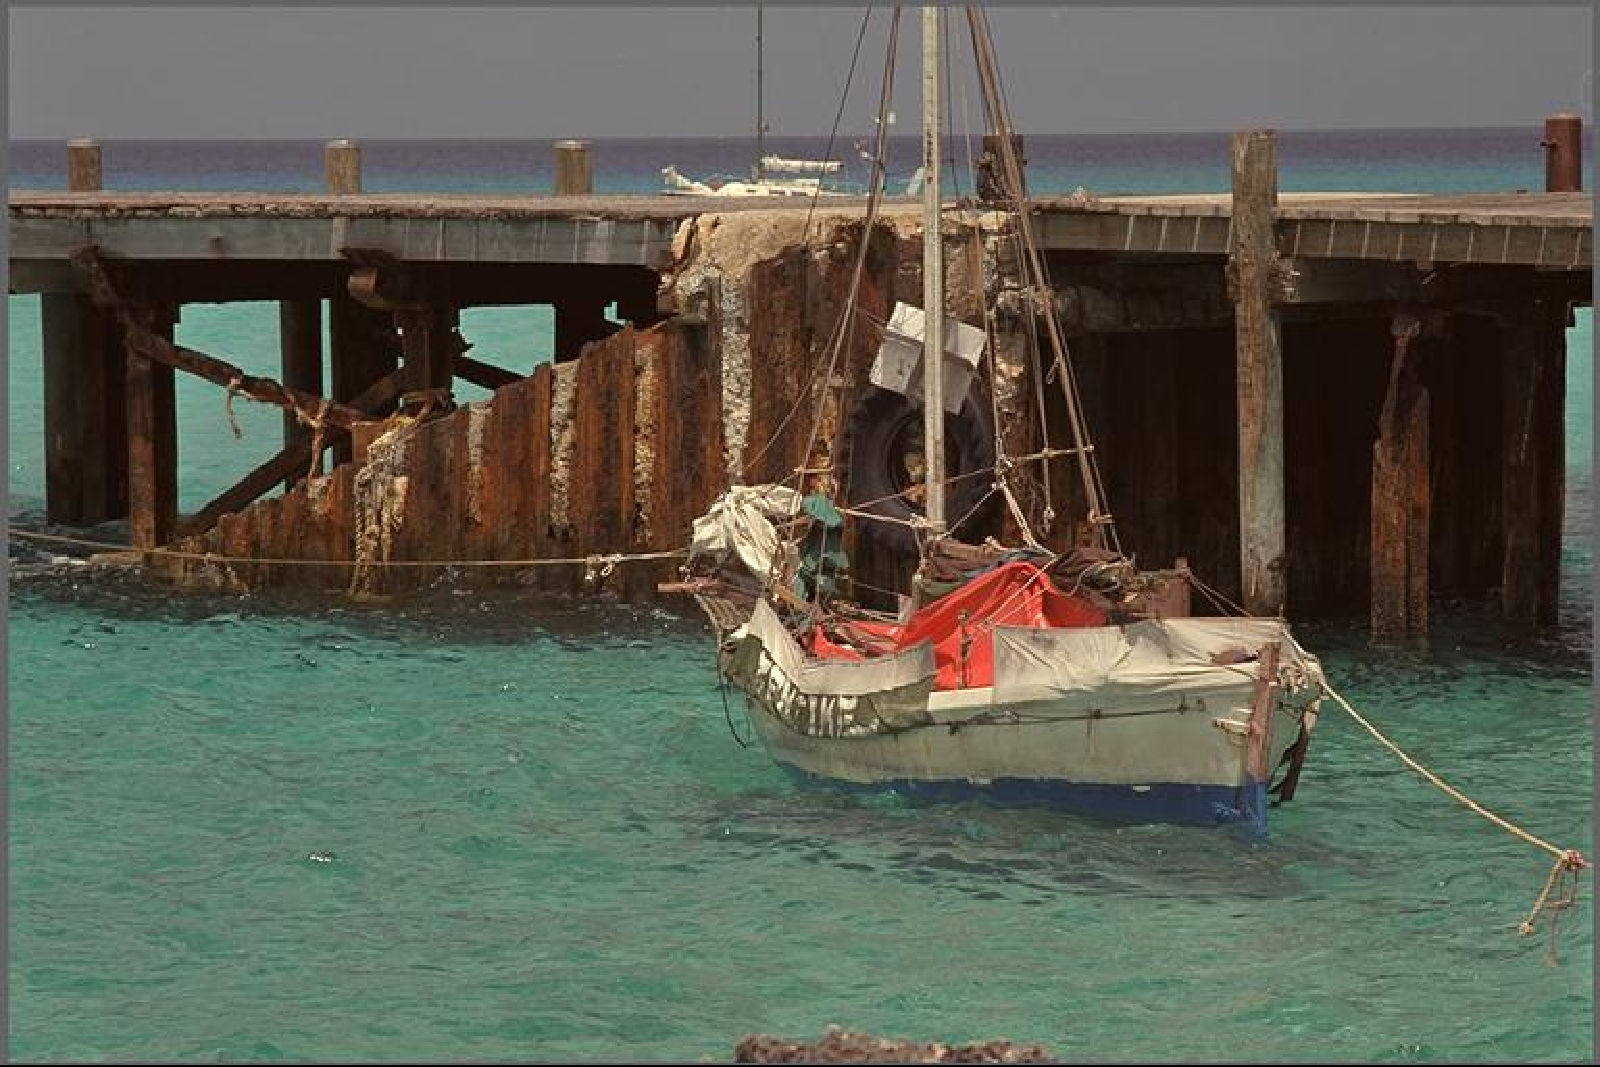
\includegraphics[width=1\textwidth]{figuras/kodim11.pdf}}
	\newline
	\subfloat[{Imagem reconstruída. Taxa: 0,741 bpp, \acrshort{psnr}: 32,190dB, \acrshort{ssim}: 0,8675.}   ]{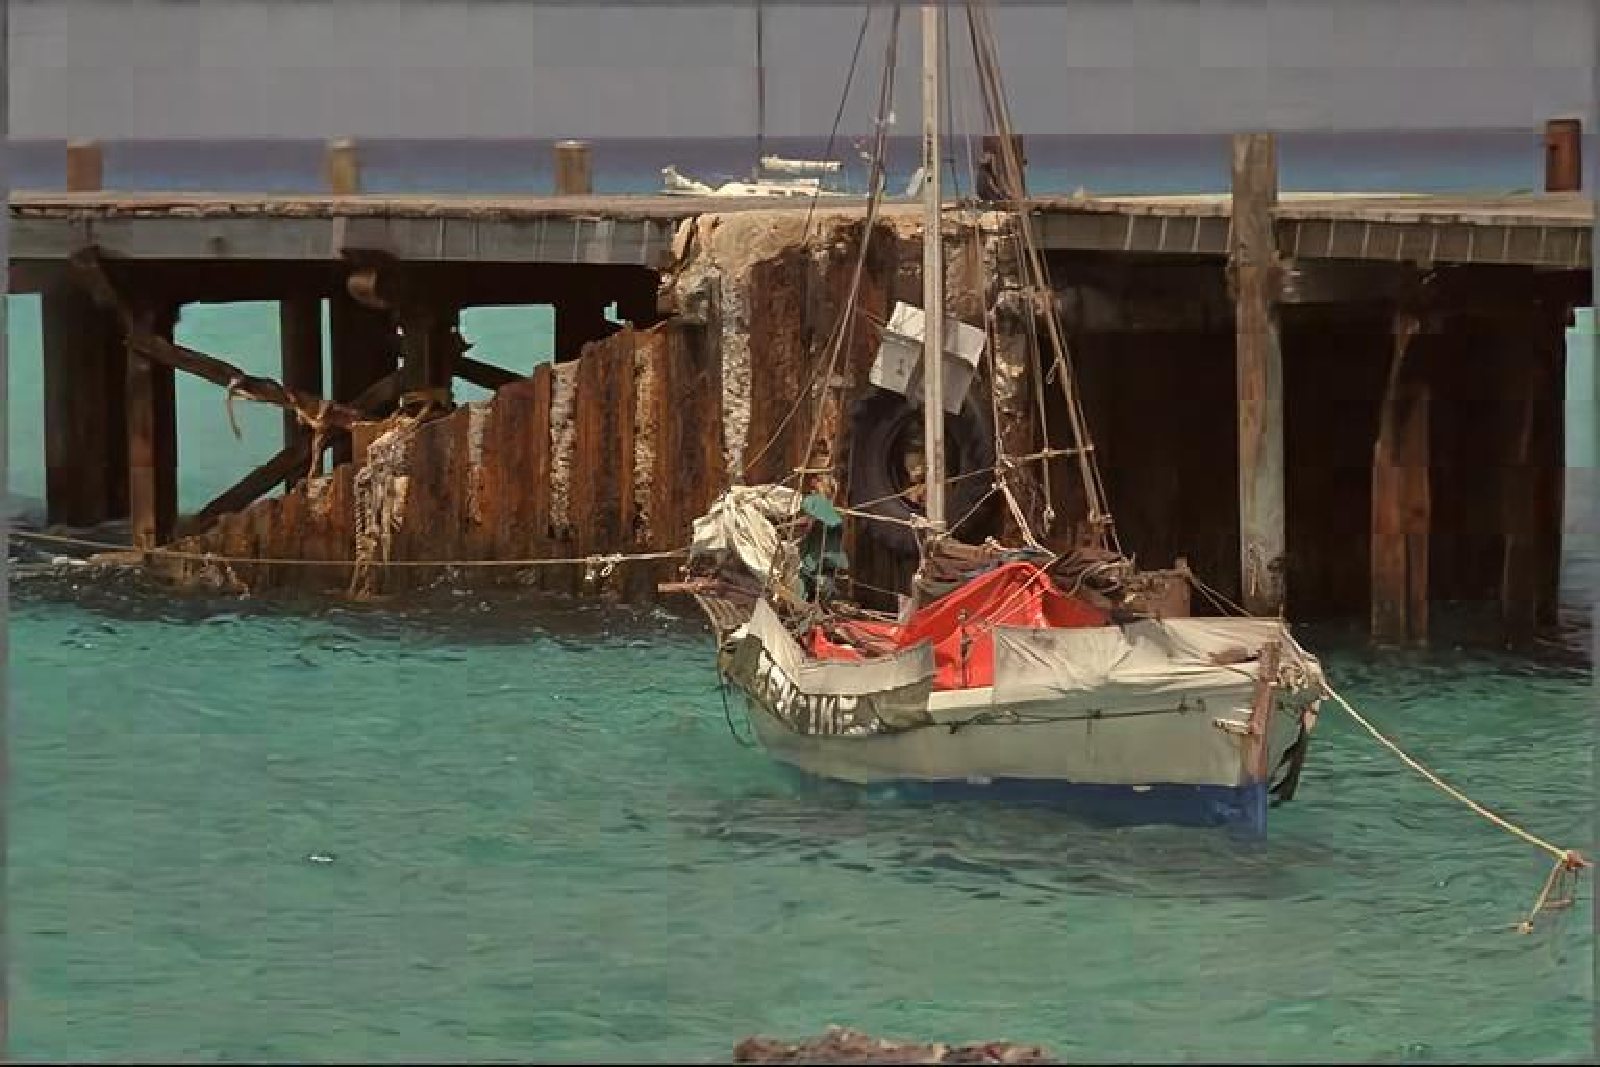
\includegraphics[width=1\textwidth]{figuras/kodim11targ_1_2431.pdf}}
	\caption[Surgimento de artefatos de blocos no método alocação de bits usando o modeloVR0]{Em (a) temos a \textit{kodim11} original. A figura (b) é uma reconstrução com o modeloVR0.}
	\label{fig:artefatos1}
\end{figure}

\begin{figure}[]
	\subfloat[Imagem reconstruída. Taxa: 0,782 bpp, \acrshort{psnr}: 32,687dB, \acrshort{ssim}: 0,8939]{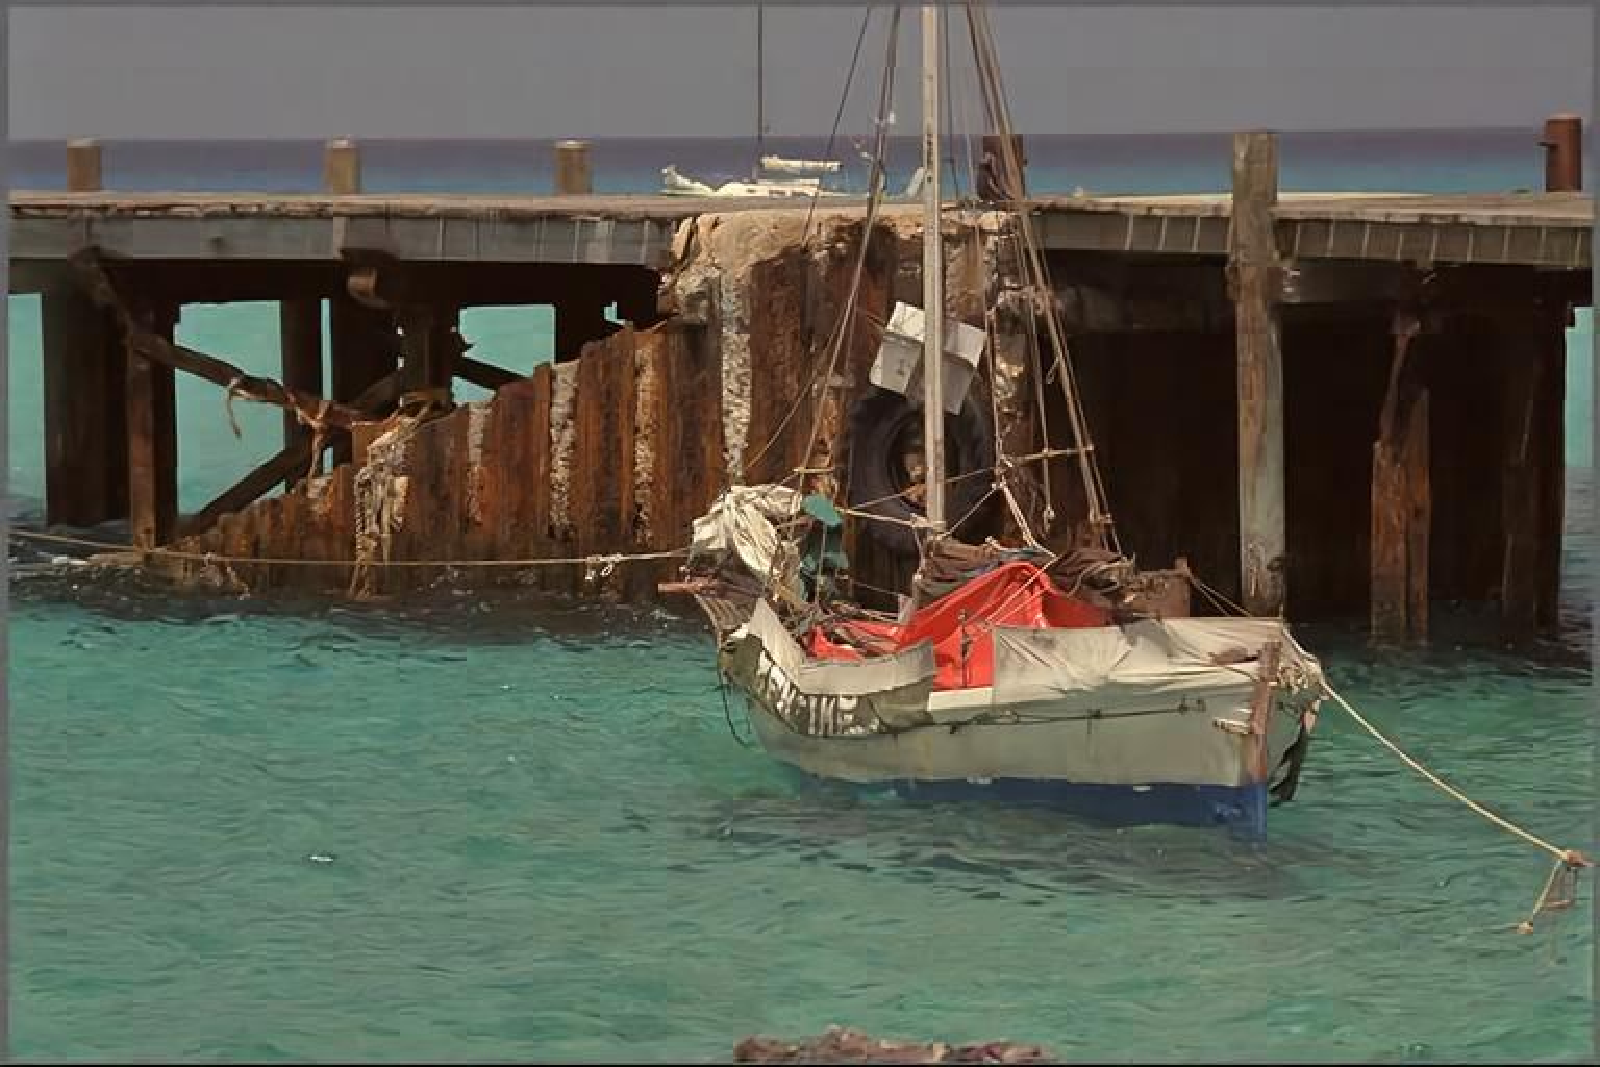
\includegraphics[width=1.0\textwidth]{figuras/kodim11targ30.pdf}}
	\newline
	\subfloat[{Imagem reconstruída. Taxa: 0,754 bpp, \acrshort{psnr}: 31,621dB, \acrshort{ssim}:0,8985 }   ]{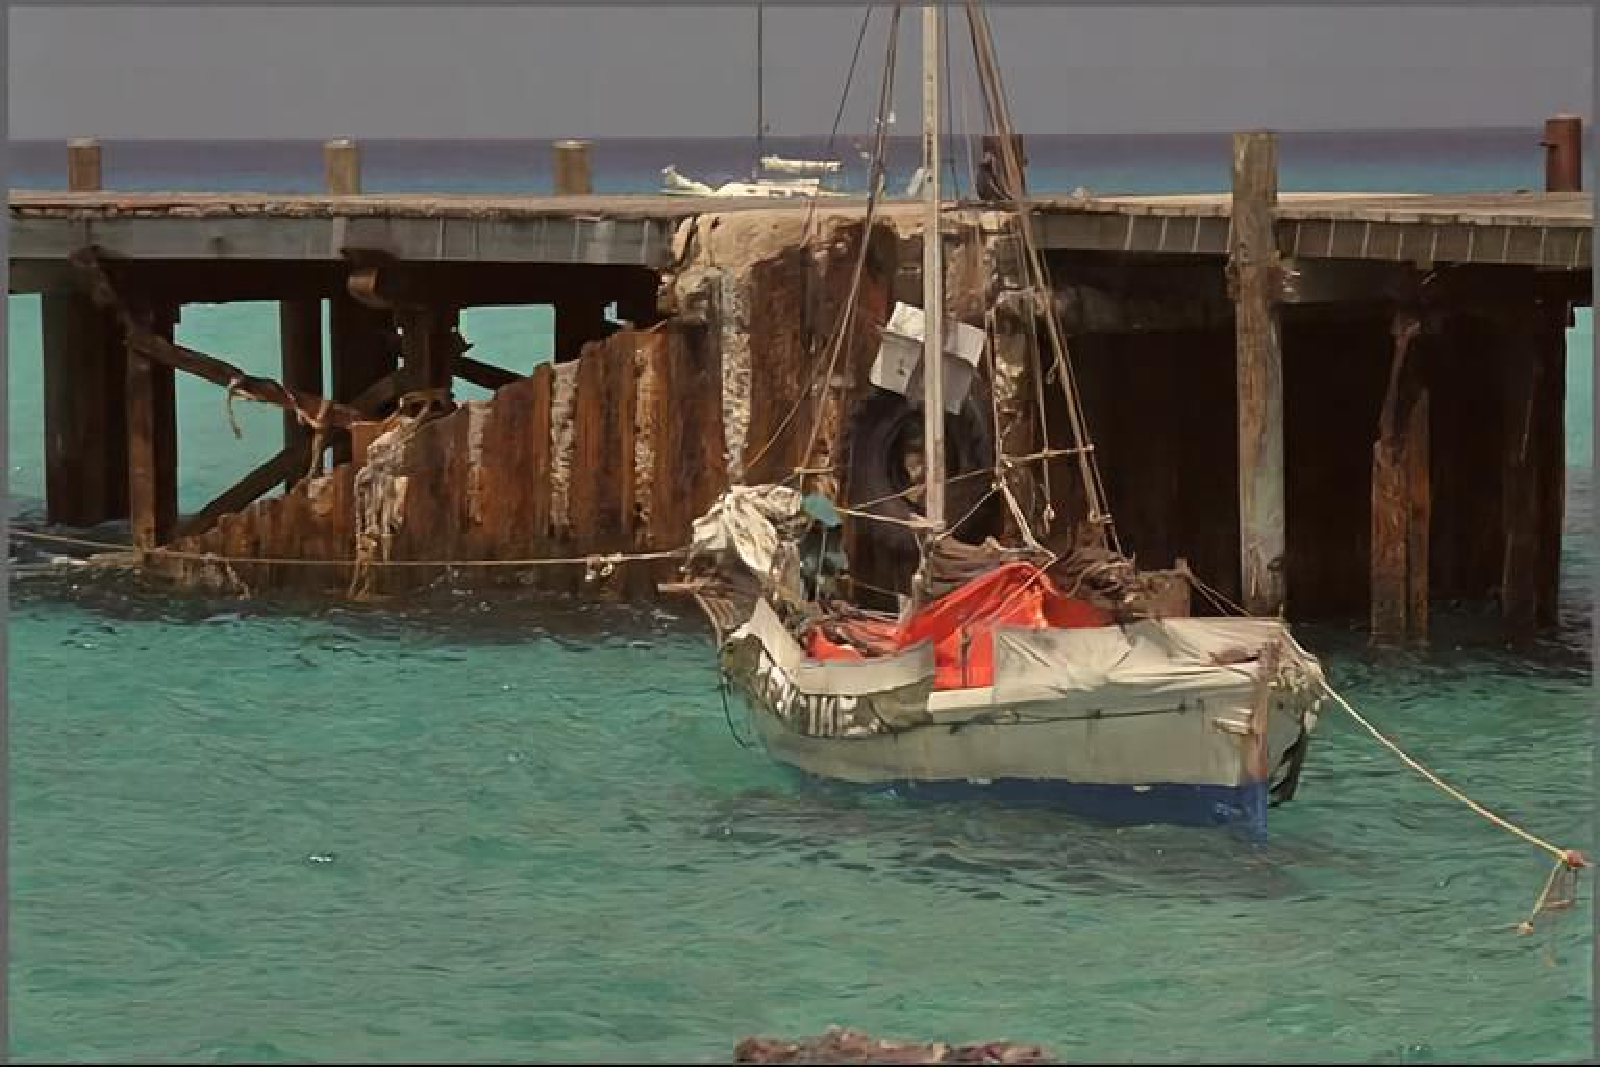
\includegraphics[width=1.0\textwidth]{figuras/kodim11it7.pdf}}
	\caption[Surgimento de artefatos de blocos no método alocação de bits usando o modeloVR]{Em (a) apresentamos a \textit{kodim11} codificada pelo modeloVR, em (b) está ilustrado sua reconstrução com o modelo (sem alocação de bits) usando 7 níveis de resíduo.}
	\label{fig:artefatos2}
\end{figure}

A Figura em \ref{fig:comp_vr} compara os modelos baseados com taxas nominais variáveis e fixas. O modeveloVR0 apresenta o pior resultado na métrica \acrshort{ssim}. Em virtude dos artefatos de blocos a qualidade perceptiva da imagem caí drasticamente. No modeloVR, o número mínimo de iterações não permite atingirmos baixas taxas de compressão. Ele supera o nosso modelo de taxas nominais fixas em \acrshort{psnr}, contudo, sofre com a perda de qualidade em \acrshort{ssim}.      

\begin{figure}
	\centering
	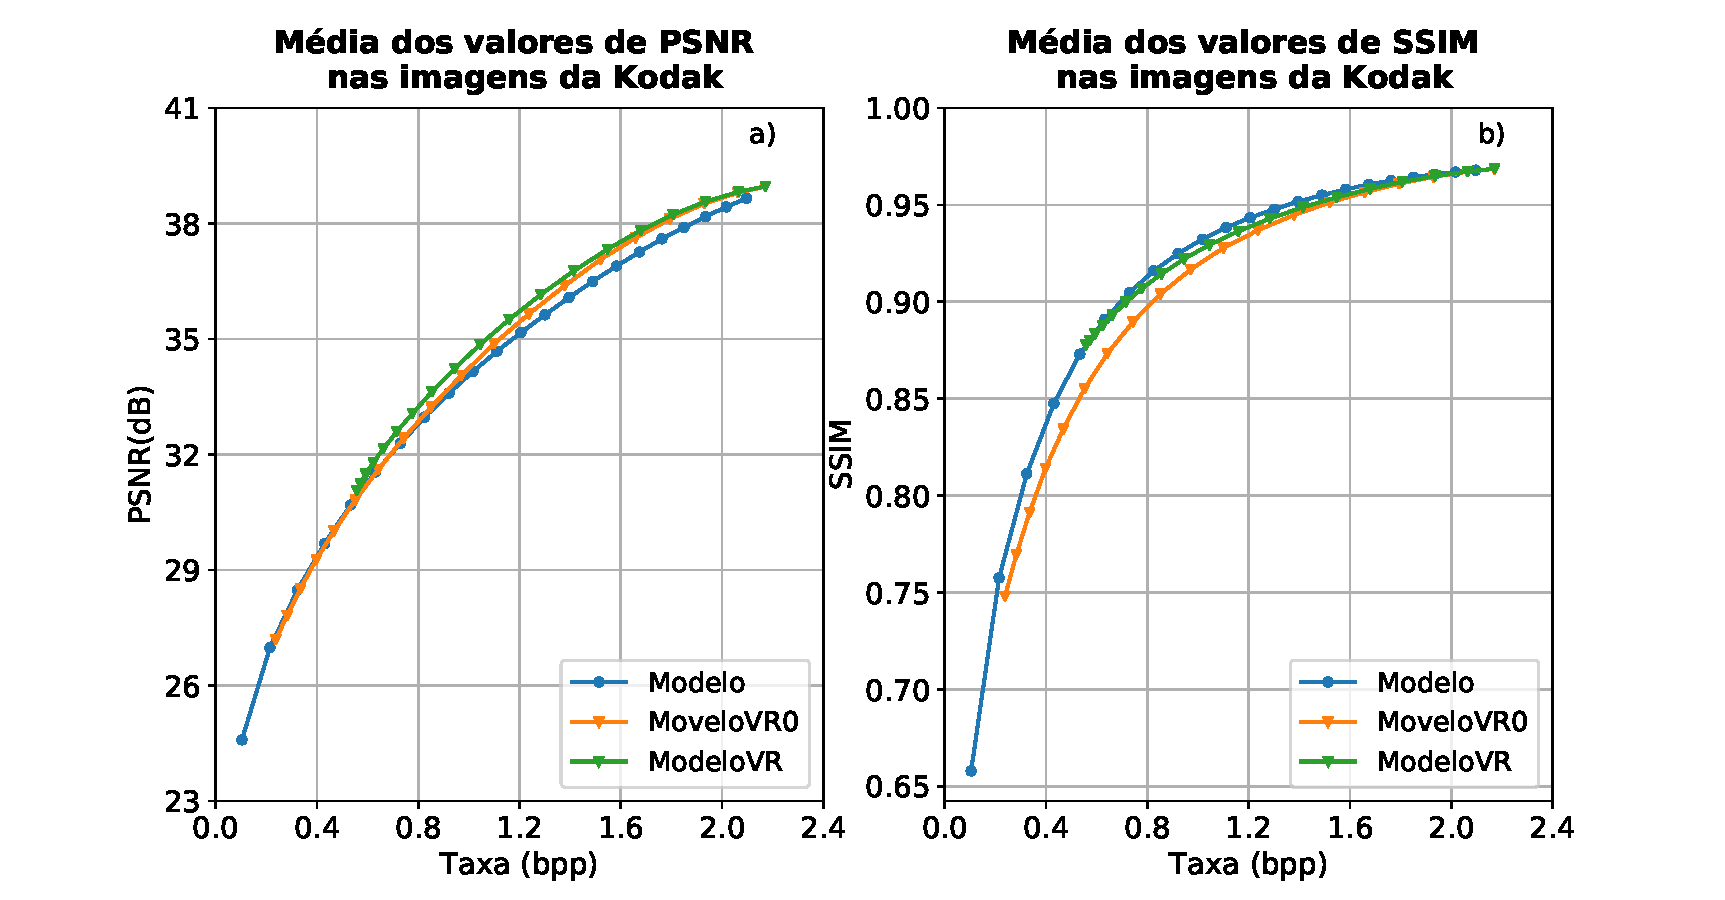
\includegraphics[width=1.0\textwidth]{figuras/com_vr.pdf}
	\caption[Comparação dos modelos de taxa variável e taxa fixa.]{Comparação dos modelos de taxa variável e de taxa fixa, ambos com codificação de entropia. A melhoria de \acrshort{psnr} nos modelos de taxa variável é acompanhada por redução de qualidade em \acrshort{ssim}.}  	
	\label{fig:comp_vr}
\end{figure}

\section{Comparação com JPEG e JPEG2000}

Nessa seção comparamos os nossos melhores resultados com o \acrshort{jpeg} e \acrshort{jpeg}2000 nas métricas \acrshort{ssim}, \acrshort{msssim} e \acrshort{psnr}. 


As Figuras em \ref{fig:comp_psnr}, \ref{fig:comp_ssim} e \ref{fig:comp_msssim} comparam os nossos melhores resultados nas abordagem usando ou não a alocação dinâmica de bits com o \acrshort{jpeg} e \acrshort{jpeg}2000. Na base de teste da Kodak, nossos modelos superam o \acrshort{jpeg} em todas as métricas apresentadas e para qualquer taxa. Em relação ao \acrshort{jpeg}2000, temos resultados competitivos, principalmente em altas taxas. Para baixas taxas o \acrshort{jpeg}2000 tem melhor desempenho.  



\begin{figure}[h]
	\centering
	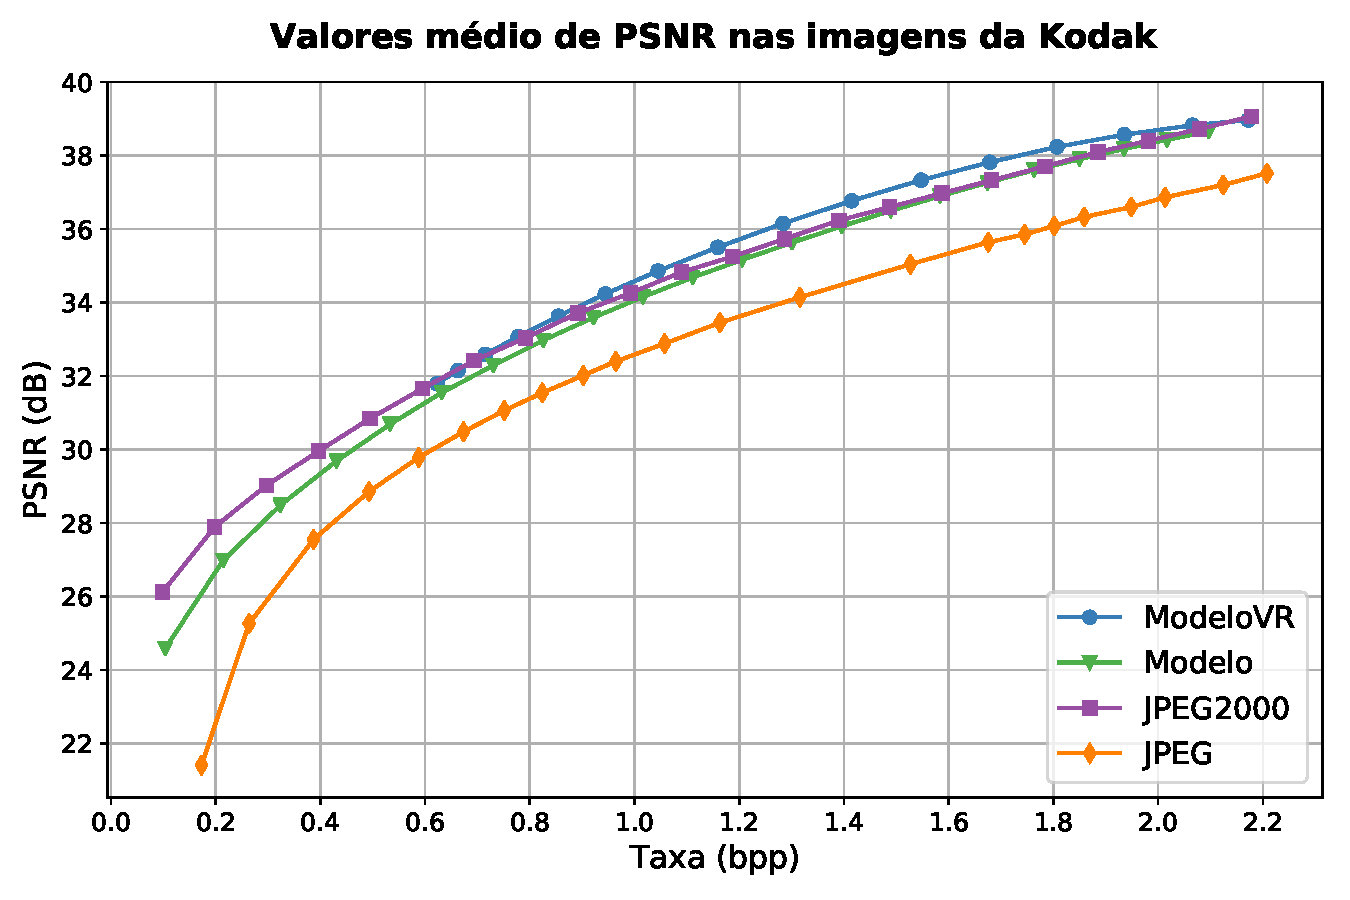
\includegraphics[width=1.0\textwidth]{figuras/comp_codecs.pdf}
	\caption[Comparações de autocodificadores com o \acrshort{jpeg} e \acrshort{jpeg}2000 em \acrshort{psnr}.]{Curvas \acrshort{psnr} $\times$ Taxa.}  	
	\label{fig:comp_psnr}
\end{figure}

\begin{figure}[h]
	\centering
	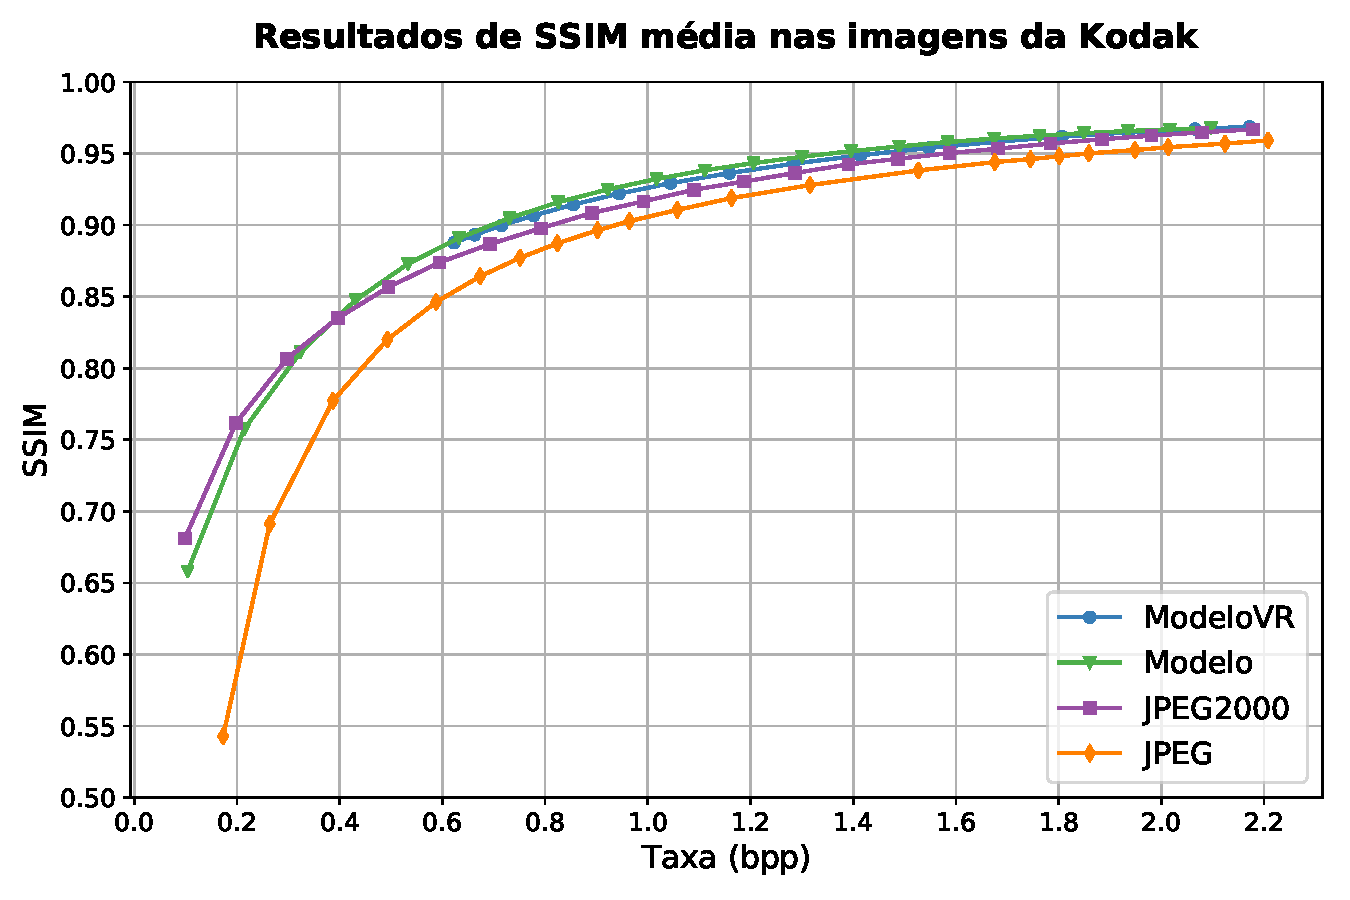
\includegraphics[width=1.0\textwidth]{figuras/comp_codecs_ssim.pdf}
	\caption[Comparações de autocodificadores com o \acrshort{jpeg} e \acrshort{jpeg}2000 em \acrshort{ssim}]{Curvas \acrshort{ssim} $\times$ Taxa.}  	
	\label{fig:comp_ssim}
\end{figure}


\begin{figure}[H]
	\centering
	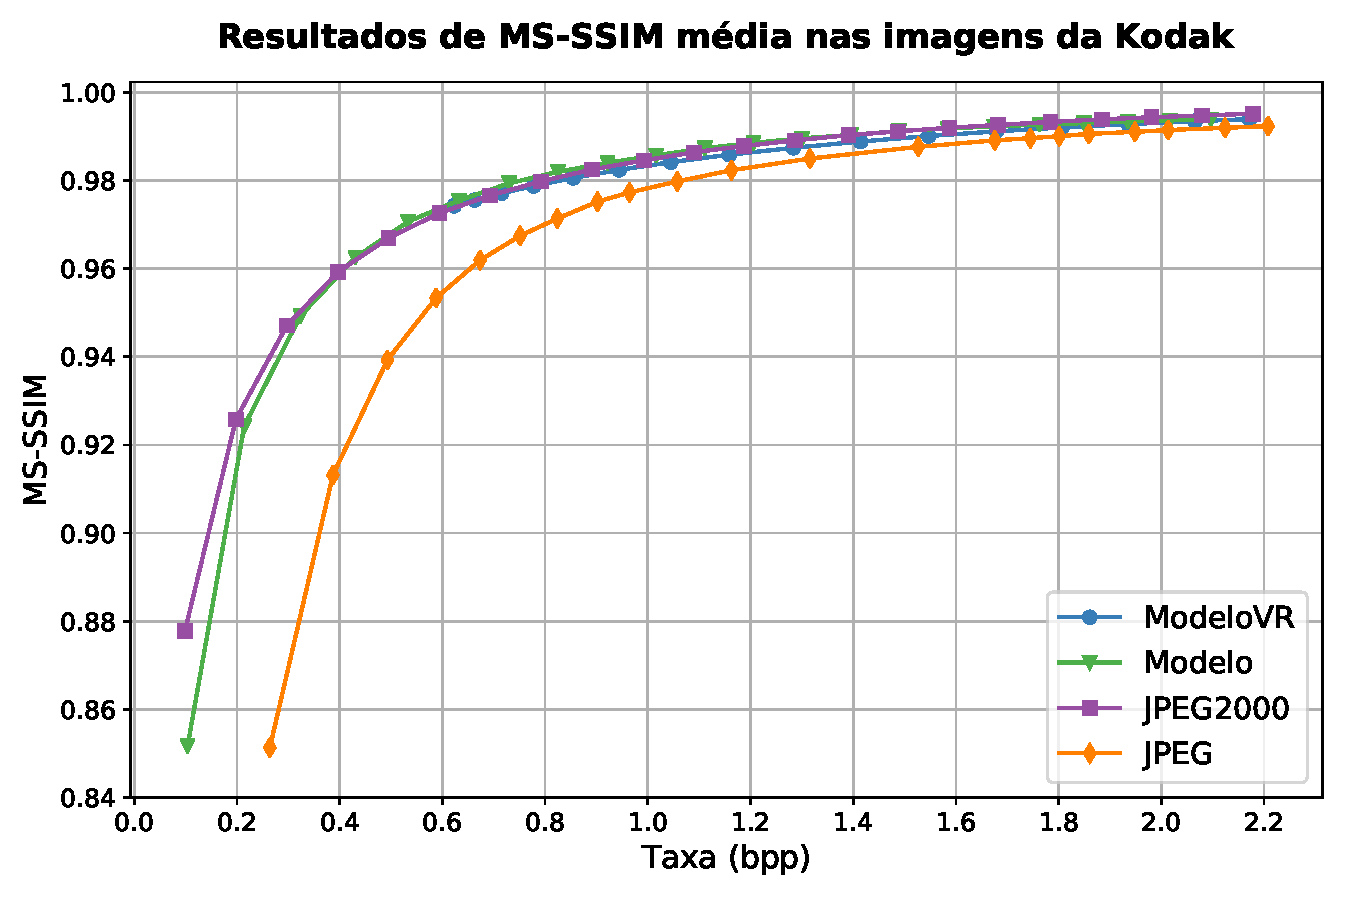
\includegraphics[width=1.0\textwidth]{figuras/comp_codecs_msssim.pdf}
	\caption[Comparações de autocodificadores com o \acrshort{jpeg} e \acrshort{jpeg}2000 em \acrshort{msssim}]{Curvas \acrshort{msssim} $\times$ Taxa.}  	
	\label{fig:comp_msssim}
\end{figure}



%\begin{figure}[h]
%	\centering
%	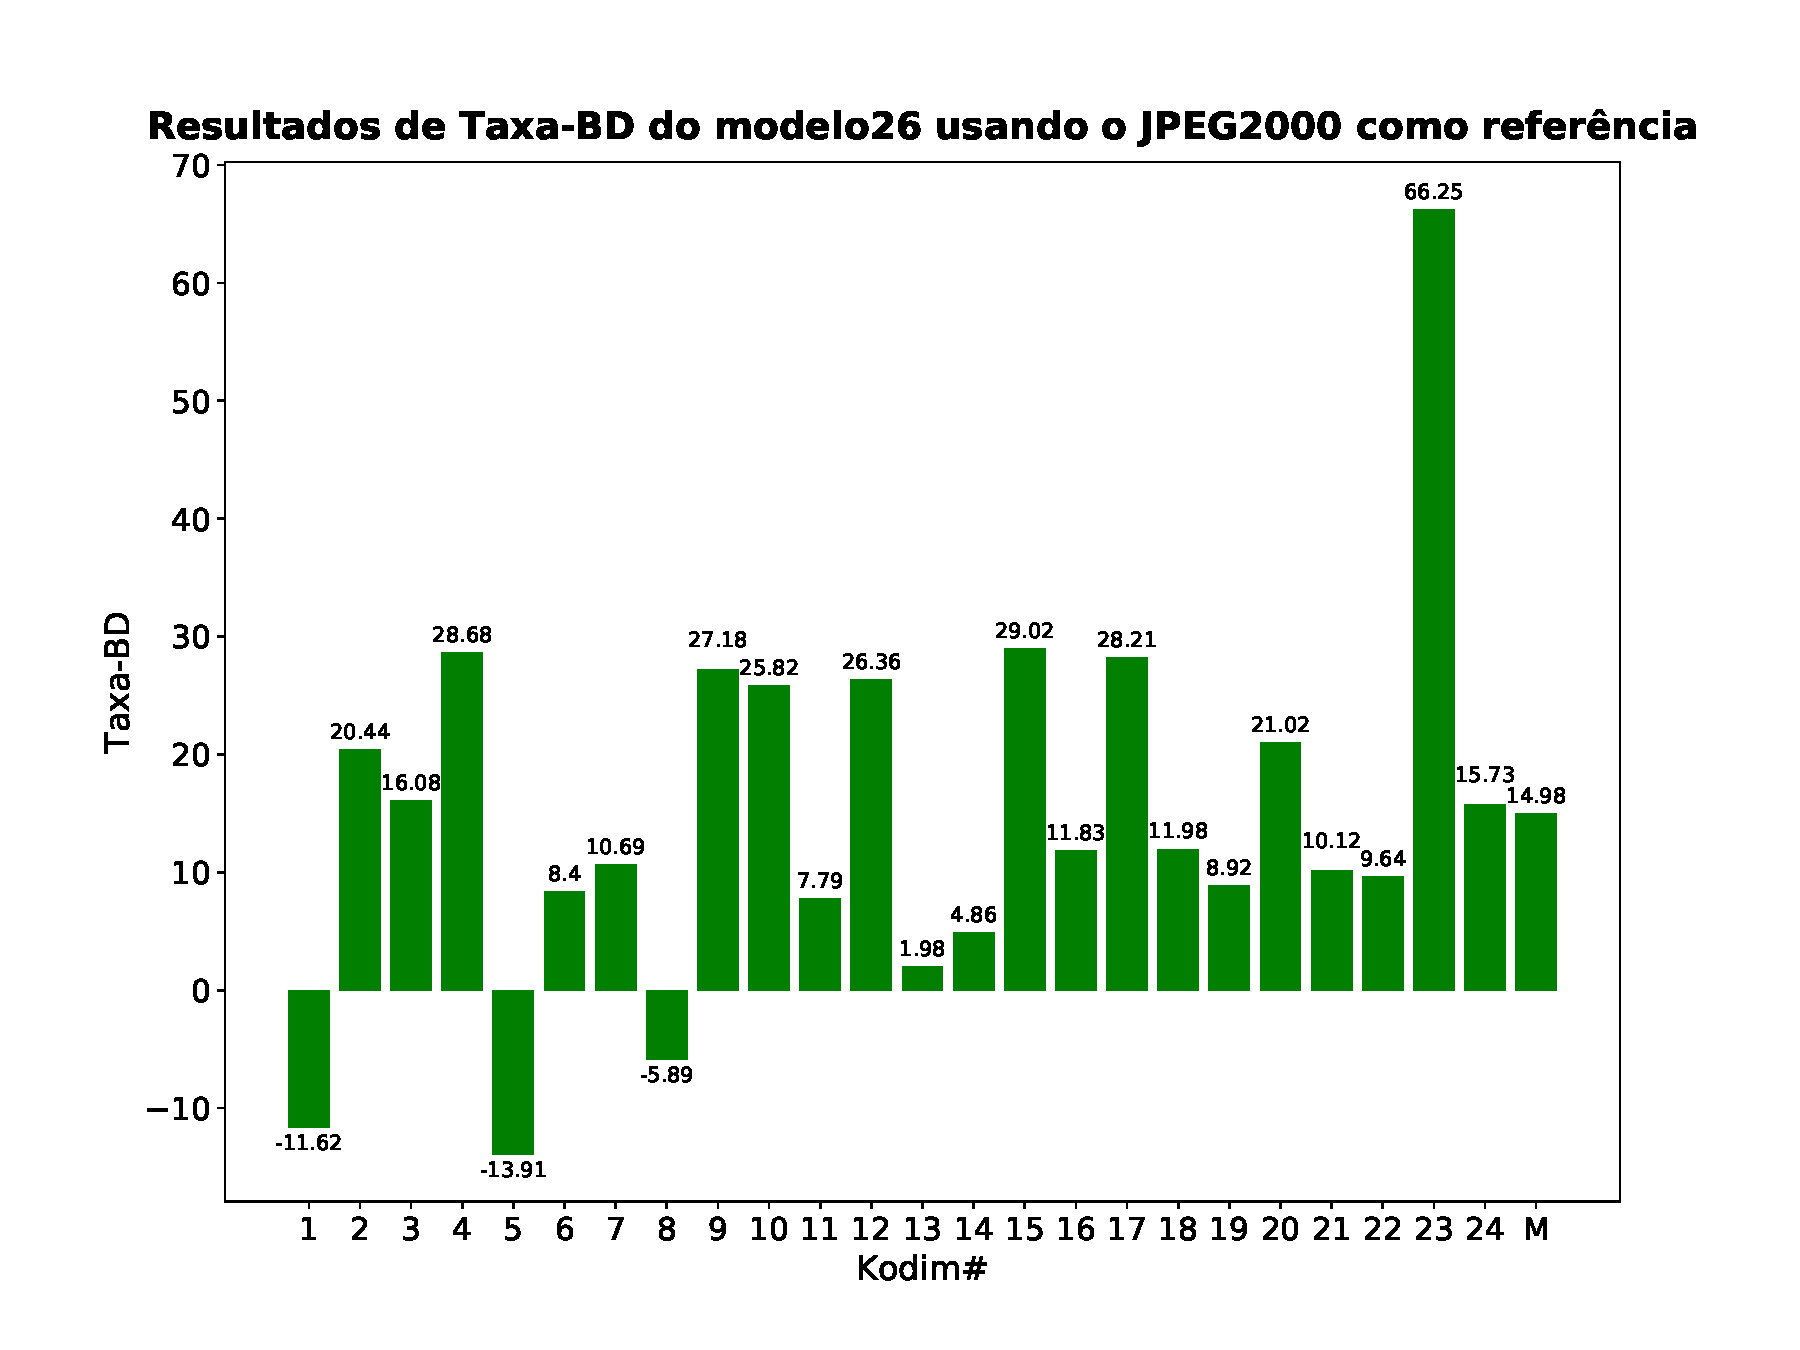
\includegraphics[width=1.0\textwidth]{figuras/bd-rate_ref_JPEG2k.pdf}
%	\caption[Comparação do modelo26 com \acrshort{jpeg}2000 em \acrshort{bdrate}]{Desempenho do nosso Modelo treinado por 26 épocas em relação ao \acrshort{jpeg}2000. Na média, estamos usando 14,98\% a mais de taxa em relação ao \acrshort{jpeg}2000 para realizar compressão em uma qualidade equivalente de \acrshort{psnr}.}  	
%	\label{fig:comp_jp2k}
%\end{figure}



%\begin{figure}[h]
%	\centering
%	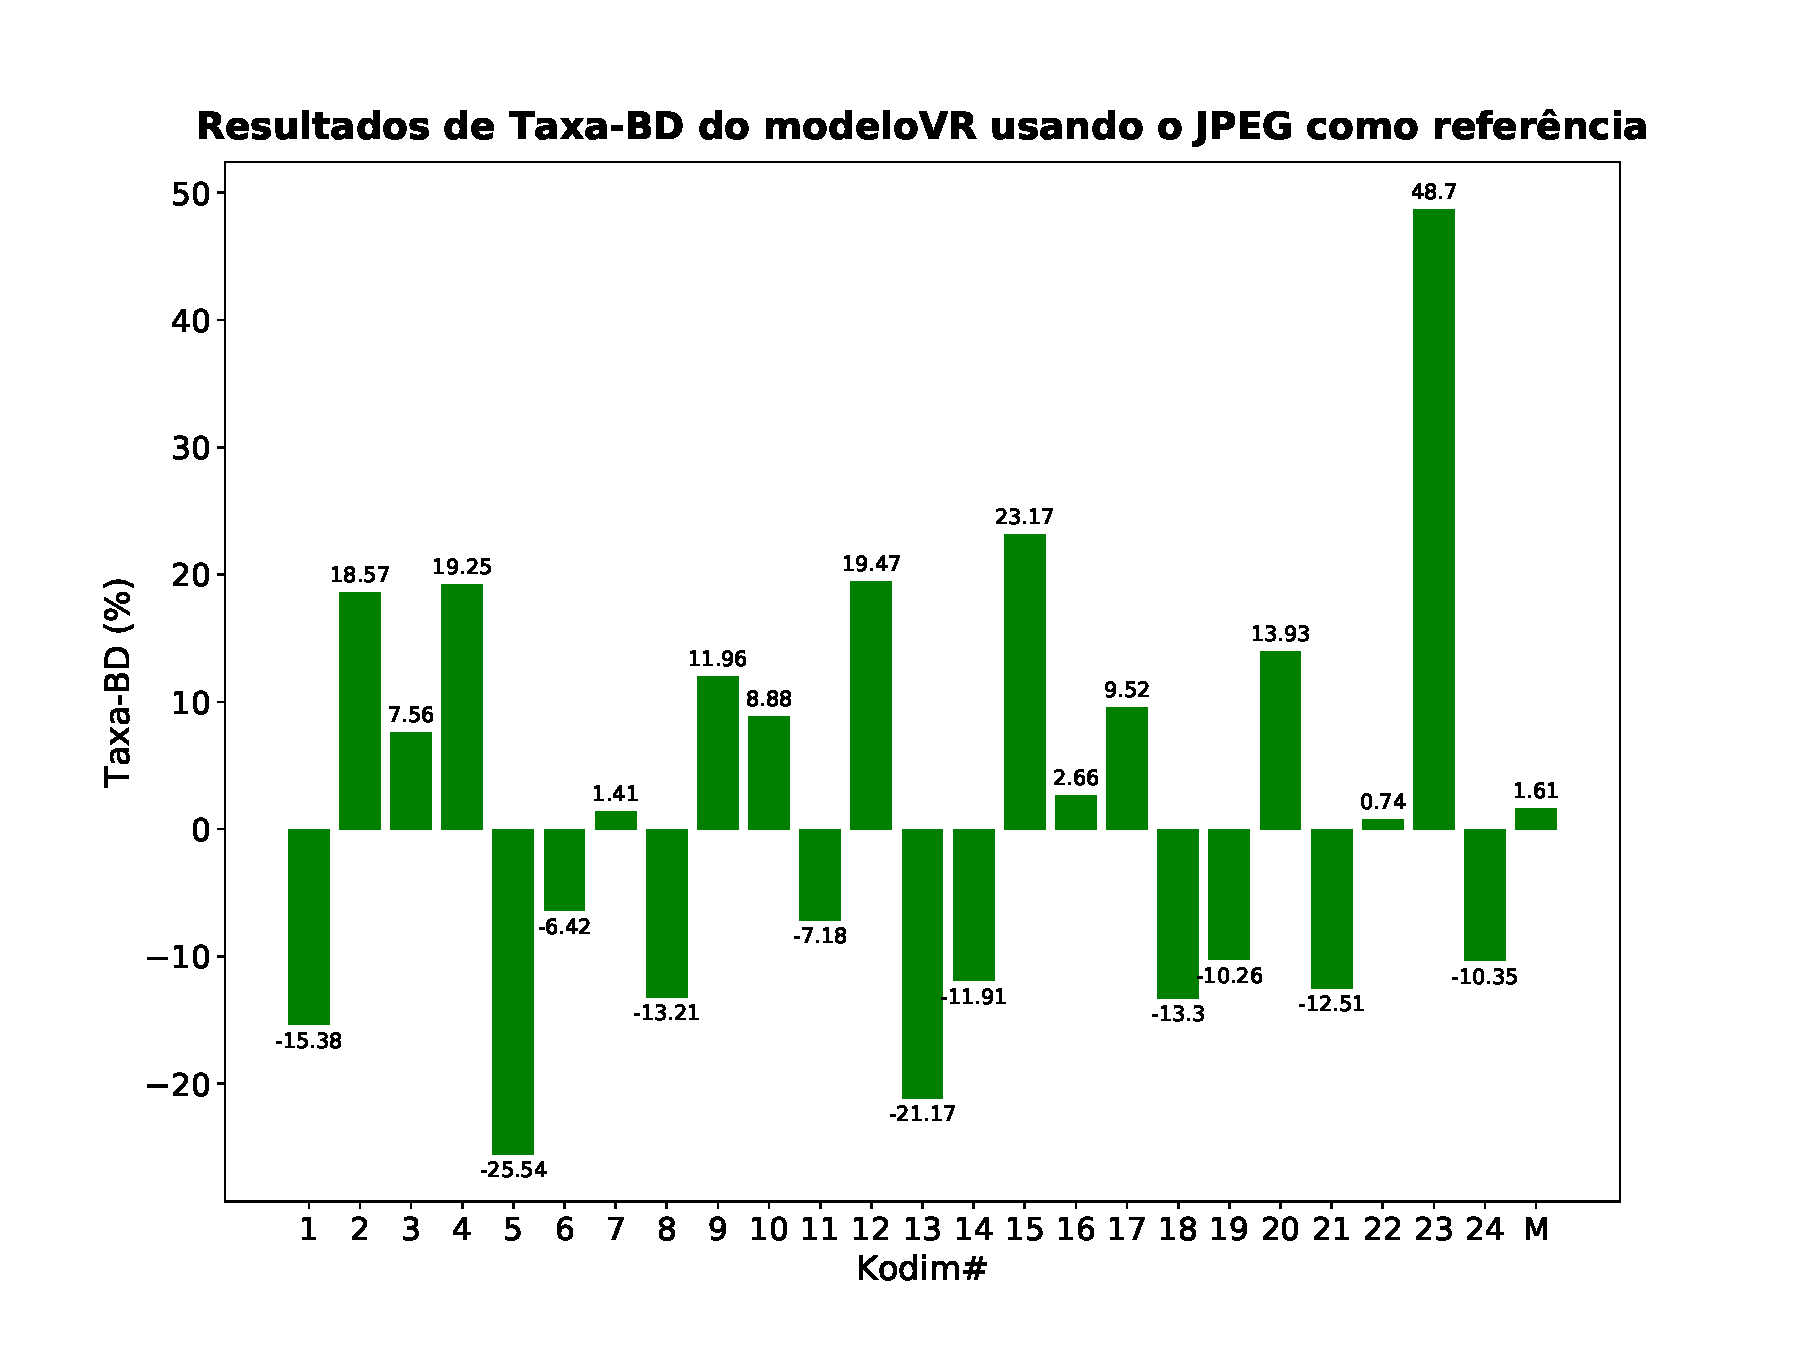
\includegraphics[width=1.0\textwidth]{figuras/bd-rate_ref_JPEG.pdf}
%	\caption[Comparação do modeloVR com \acrshort{jpeg}2000 em \acrshort{bdrate}]{Desempenho do nosso modelo de taxa variável em relação ao \acrshort{jpeg}2000. Aqui, nossos resultados se mostram mais competitivos. Em 11 imagens da Kodak economizamos bits, nas demais consumimos mais bits do que seria requisitado pelo \acrshort{jpeg}2000.}  	
%	\label{fig:comp_jp2k_vr}
%\end{figure}






